% Options for packages loaded elsewhere
\PassOptionsToPackage{unicode}{hyperref}
\PassOptionsToPackage{hyphens}{url}
\documentclass[
]{article}
\usepackage{xcolor}
\usepackage{amsmath,amssymb}
\setcounter{secnumdepth}{-\maxdimen} % remove section numbering
\usepackage{iftex}
\ifPDFTeX
  \usepackage[T1]{fontenc}
  \usepackage[utf8]{inputenc}
  \usepackage{textcomp} % provide euro and other symbols
\else % if luatex or xetex
  \usepackage{unicode-math} % this also loads fontspec
  \defaultfontfeatures{Scale=MatchLowercase}
  \defaultfontfeatures[\rmfamily]{Ligatures=TeX,Scale=1}
\fi
\usepackage{lmodern}
\ifPDFTeX\else
  % xetex/luatex font selection
\fi
% Use upquote if available, for straight quotes in verbatim environments
\IfFileExists{upquote.sty}{\usepackage{upquote}}{}
\IfFileExists{microtype.sty}{% use microtype if available
  \usepackage[]{microtype}
  \UseMicrotypeSet[protrusion]{basicmath} % disable protrusion for tt fonts
}{}
\makeatletter
\@ifundefined{KOMAClassName}{% if non-KOMA class
  \IfFileExists{parskip.sty}{%
    \usepackage{parskip}
  }{% else
    \setlength{\parindent}{0pt}
    \setlength{\parskip}{6pt plus 2pt minus 1pt}}
}{% if KOMA class
  \KOMAoptions{parskip=half}}
\makeatother
\usepackage{color}
\usepackage{fancyvrb}
\newcommand{\VerbBar}{|}
\newcommand{\VERB}{\Verb[commandchars=\\\{\}]}
\DefineVerbatimEnvironment{Highlighting}{Verbatim}{commandchars=\\\{\}}
% Add ',fontsize=\small' for more characters per line
\newenvironment{Shaded}{}{}
\newcommand{\AlertTok}[1]{\textcolor[rgb]{1.00,0.00,0.00}{\textbf{#1}}}
\newcommand{\AnnotationTok}[1]{\textcolor[rgb]{0.38,0.63,0.69}{\textbf{\textit{#1}}}}
\newcommand{\AttributeTok}[1]{\textcolor[rgb]{0.49,0.56,0.16}{#1}}
\newcommand{\BaseNTok}[1]{\textcolor[rgb]{0.25,0.63,0.44}{#1}}
\newcommand{\BuiltInTok}[1]{\textcolor[rgb]{0.00,0.50,0.00}{#1}}
\newcommand{\CharTok}[1]{\textcolor[rgb]{0.25,0.44,0.63}{#1}}
\newcommand{\CommentTok}[1]{\textcolor[rgb]{0.38,0.63,0.69}{\textit{#1}}}
\newcommand{\CommentVarTok}[1]{\textcolor[rgb]{0.38,0.63,0.69}{\textbf{\textit{#1}}}}
\newcommand{\ConstantTok}[1]{\textcolor[rgb]{0.53,0.00,0.00}{#1}}
\newcommand{\ControlFlowTok}[1]{\textcolor[rgb]{0.00,0.44,0.13}{\textbf{#1}}}
\newcommand{\DataTypeTok}[1]{\textcolor[rgb]{0.56,0.13,0.00}{#1}}
\newcommand{\DecValTok}[1]{\textcolor[rgb]{0.25,0.63,0.44}{#1}}
\newcommand{\DocumentationTok}[1]{\textcolor[rgb]{0.73,0.13,0.13}{\textit{#1}}}
\newcommand{\ErrorTok}[1]{\textcolor[rgb]{1.00,0.00,0.00}{\textbf{#1}}}
\newcommand{\ExtensionTok}[1]{#1}
\newcommand{\FloatTok}[1]{\textcolor[rgb]{0.25,0.63,0.44}{#1}}
\newcommand{\FunctionTok}[1]{\textcolor[rgb]{0.02,0.16,0.49}{#1}}
\newcommand{\ImportTok}[1]{\textcolor[rgb]{0.00,0.50,0.00}{\textbf{#1}}}
\newcommand{\InformationTok}[1]{\textcolor[rgb]{0.38,0.63,0.69}{\textbf{\textit{#1}}}}
\newcommand{\KeywordTok}[1]{\textcolor[rgb]{0.00,0.44,0.13}{\textbf{#1}}}
\newcommand{\NormalTok}[1]{#1}
\newcommand{\OperatorTok}[1]{\textcolor[rgb]{0.40,0.40,0.40}{#1}}
\newcommand{\OtherTok}[1]{\textcolor[rgb]{0.00,0.44,0.13}{#1}}
\newcommand{\PreprocessorTok}[1]{\textcolor[rgb]{0.74,0.48,0.00}{#1}}
\newcommand{\RegionMarkerTok}[1]{#1}
\newcommand{\SpecialCharTok}[1]{\textcolor[rgb]{0.25,0.44,0.63}{#1}}
\newcommand{\SpecialStringTok}[1]{\textcolor[rgb]{0.73,0.40,0.53}{#1}}
\newcommand{\StringTok}[1]{\textcolor[rgb]{0.25,0.44,0.63}{#1}}
\newcommand{\VariableTok}[1]{\textcolor[rgb]{0.10,0.09,0.49}{#1}}
\newcommand{\VerbatimStringTok}[1]{\textcolor[rgb]{0.25,0.44,0.63}{#1}}
\newcommand{\WarningTok}[1]{\textcolor[rgb]{0.38,0.63,0.69}{\textbf{\textit{#1}}}}
\usepackage{longtable,booktabs,array}
\usepackage{calc} % for calculating minipage widths
% Correct order of tables after \paragraph or \subparagraph
\usepackage{etoolbox}
\makeatletter
\patchcmd\longtable{\par}{\if@noskipsec\mbox{}\fi\par}{}{}
\makeatother
% Allow footnotes in longtable head/foot
\IfFileExists{footnotehyper.sty}{\usepackage{footnotehyper}}{\usepackage{footnote}}
\makesavenoteenv{longtable}
\usepackage{graphicx}
\makeatletter
\newsavebox\pandoc@box
\newcommand*\pandocbounded[1]{% scales image to fit in text height/width
  \sbox\pandoc@box{#1}%
  \Gscale@div\@tempa{\textheight}{\dimexpr\ht\pandoc@box+\dp\pandoc@box\relax}%
  \Gscale@div\@tempb{\linewidth}{\wd\pandoc@box}%
  \ifdim\@tempb\p@<\@tempa\p@\let\@tempa\@tempb\fi% select the smaller of both
  \ifdim\@tempa\p@<\p@\scalebox{\@tempa}{\usebox\pandoc@box}%
  \else\usebox{\pandoc@box}%
  \fi%
}
% Set default figure placement to htbp
\def\fps@figure{htbp}
\makeatother
\usepackage{svg}
\ifLuaTeX
\usepackage[bidi=basic]{babel}
\else
\usepackage[bidi=default]{babel}
\fi
\babelprovide[main,import]{french}
% get rid of language-specific shorthands (see #6817):
\let\LanguageShortHands\languageshorthands
\def\languageshorthands#1{}
\setlength{\emergencystretch}{3em} % prevent overfull lines
\providecommand{\tightlist}{%
  \setlength{\itemsep}{0pt}\setlength{\parskip}{0pt}}
\usepackage{bookmark}
\IfFileExists{xurl.sty}{\usepackage{xurl}}{} % add URL line breaks if available
\urlstyle{same}
\hypersetup{
  pdftitle={6~ Classifications d'images supervisées -- Traitement d\textquotesingle images satellites avec Python},
  pdflang={fr},
  hidelinks,
  pdfcreator={LaTeX via pandoc}}

\title{6~ Classifications d'images supervisées -- Traitement
d\textquotesingle images satellites avec Python}
\author{}
\date{}

\begin{document}
\maketitle

\phantomsection\label{quarto-document-content}
\phantomsection\label{title-block-header}
\section{\texorpdfstring{\protect\hypertarget{sec-chap05}{}{{6}~
{Classifications d'images
supervisées}}}{6~ Classifications d'images supervisées}}\label{classifications-dimages-supervisuxe9es}

\subsection{\texorpdfstring{{6.1} {🚀}
Préambule}{6.1 🚀 Préambule}}\label{pruxe9ambule}

Assurez-vous de lire ce préambule avant d'exécutez le reste du notebook.

\subsubsection{\texorpdfstring{{6.1.1} {🎯}
Objectifs}{6.1.1 🎯 Objectifs}}\label{objectifs}

Dans ce chapitre, nous ferons une introduction générale à
l'apprentissage automatique et abordons quelques techniques
fondamentales. La librairie centrale utilisée dans ce chapitre sera
\href{https://scikit-learn.org/}{\texttt{sickit-learn}}. Ce chapitre est
aussi disponible sous la forme d'un notebook Python sur Google Colab:

\href{https://colab.research.google.com/github/sfoucher/TraitementImagesPythonVol1/blob/main/notebooks/05-ClassificationsSupervisees.ipynb}{\pandocbounded{\includesvg[keepaspectratio]{images/colab-badge.svg}}}

\subsubsection{\texorpdfstring{{6.1.2}
Librairies}{6.1.2 Librairies}}\label{librairies}

Les librairies utilisées dans ce chapitre sont les suivantes:

\begin{itemize}
\item
  \href{https://scipy.org/}{SciPy}
\item
  \href{https://numpy.org/}{NumPy}
\item
  \href{https://pypi.org/project/opencv-python/}{opencv-python · PyPI}
\item
  \href{https://scikit-image.org/}{scikit-image}
\item
  \href{https://rasterio.readthedocs.io/en/stable/}{Rasterio}
\item
  \href{https://docs.xarray.dev/en/stable/}{xarray}
\item
  \href{https://corteva.github.io/rioxarray/stable/index.html}{rioxarray}
\item
  \href{https://geopandas.org}{geopandas}
\item
  \href{https://scikit-learn.org/}{scikit-learn}
\end{itemize}

Dans l'environnement Google Colab, seul \texttt{rioxarray} et
\texttt{xrscipy} doit être installés:

\phantomsection\label{3cf35c25}
\phantomsection\label{cb1}
\begin{Shaded}
\begin{Highlighting}[]
\OperatorTok{\%\%}\NormalTok{capture}
\OperatorTok{!}\NormalTok{pip install }\OperatorTok{{-}}\NormalTok{qU matplotlib rioxarray xrscipy}
\end{Highlighting}
\end{Shaded}

Vérifier les importations nécessaires en premier:

\phantomsection\label{1725a255}
\phantomsection\label{cb2}
\begin{Shaded}
\begin{Highlighting}[]
\ImportTok{import}\NormalTok{ numpy }\ImportTok{as}\NormalTok{ np}
\ImportTok{import}\NormalTok{ rioxarray }\ImportTok{as}\NormalTok{ rxr}
\ImportTok{from}\NormalTok{ scipy }\ImportTok{import}\NormalTok{ signal}
\ImportTok{import}\NormalTok{ xarray }\ImportTok{as}\NormalTok{ xr}
\ImportTok{import}\NormalTok{ rasterio}
\ImportTok{import}\NormalTok{ xrscipy}
\ImportTok{import}\NormalTok{ matplotlib.pyplot }\ImportTok{as}\NormalTok{ plt}
\ImportTok{from}\NormalTok{ matplotlib.colors }\ImportTok{import}\NormalTok{ ListedColormap}
\ImportTok{import}\NormalTok{ geopandas}
\ImportTok{from}\NormalTok{ shapely.geometry }\ImportTok{import}\NormalTok{ Point}
\ImportTok{import}\NormalTok{ pandas }\ImportTok{as}\NormalTok{ pd}
\ImportTok{from}\NormalTok{ numba }\ImportTok{import}\NormalTok{ jit}
\ImportTok{from}\NormalTok{ sklearn.neighbors }\ImportTok{import}\NormalTok{ KNeighborsClassifier}
\ImportTok{from}\NormalTok{ sklearn.model\_selection }\ImportTok{import}\NormalTok{ train\_test\_split}
\ImportTok{from}\NormalTok{ sklearn.pipeline }\ImportTok{import}\NormalTok{ Pipeline}
\ImportTok{from}\NormalTok{ sklearn.metrics }\ImportTok{import}\NormalTok{ confusion\_matrix, classification\_report, ConfusionMatrixDisplay}
\ImportTok{from}\NormalTok{ sklearn.preprocessing }\ImportTok{import}\NormalTok{ StandardScaler}
\ImportTok{from}\NormalTok{ sklearn.inspection }\ImportTok{import}\NormalTok{ DecisionBoundaryDisplay}
\ImportTok{from}\NormalTok{ sklearn.discriminant\_analysis }\ImportTok{import}\NormalTok{ LinearDiscriminantAnalysis, QuadraticDiscriminantAnalysis}
\ImportTok{from}\NormalTok{ sklearn.datasets }\ImportTok{import}\NormalTok{ make\_blobs, make\_classification, make\_gaussian\_quantiles}
\end{Highlighting}
\end{Shaded}

\subsubsection{\texorpdfstring{{6.1.3} Images
utilisées}{6.1.3 Images utilisées}}\label{images-utilisuxe9es}

Nous allons utilisez les images suivantes dans ce chapitre:

\phantomsection\label{669d08f3}
\phantomsection\label{cb3}
\begin{Shaded}
\begin{Highlighting}[]
\OperatorTok{\%\%}\NormalTok{capture}
\ImportTok{import}\NormalTok{ gdown}

\NormalTok{gdown.download(}\StringTok{\textquotesingle{}https://drive.google.com/uc?export=download\&confirm=pbef\&id=1a6Ypg0g1Oy4AJt9XWKWfnR12NW1XhNg\_\textquotesingle{}}\NormalTok{, output}\OperatorTok{=} \StringTok{\textquotesingle{}RGBNIR\_of\_S2A.tif\textquotesingle{}}\NormalTok{)}
\NormalTok{gdown.download(}\StringTok{\textquotesingle{}https://drive.google.com/uc?export=download\&confirm=pbef\&id=1a4PQ68Ru8zBphbQ22j0sgJ4D2quw{-}Wo6\textquotesingle{}}\NormalTok{, output}\OperatorTok{=} \StringTok{\textquotesingle{}landsat7.tif\textquotesingle{}}\NormalTok{)}
\NormalTok{gdown.download(}\StringTok{\textquotesingle{}https://drive.google.com/uc?export=download\&confirm=pbef\&id=1\_zwCLN{-}x7XJcNHJCH6Z8upEdUXtVtvs1\textquotesingle{}}\NormalTok{, output}\OperatorTok{=} \StringTok{\textquotesingle{}berkeley.jpg\textquotesingle{}}\NormalTok{)}
\NormalTok{gdown.download(}\StringTok{\textquotesingle{}https://drive.google.com/uc?export=download\&confirm=pbef\&id=1dM6IVqjba6GHwTLmI7CpX8GP2z5txUq6\textquotesingle{}}\NormalTok{, output}\OperatorTok{=} \StringTok{\textquotesingle{}SAR.tif\textquotesingle{}}\NormalTok{)}
\NormalTok{gdown.download(}\StringTok{\textquotesingle{}https://drive.google.com/uc?export=download\&confirm=pbef\&id=1aAq7crc\_LoaLC3kG3HkQ6Fv5JfG0mswg\textquotesingle{}}\NormalTok{, output}\OperatorTok{=} \StringTok{\textquotesingle{}carte.tif\textquotesingle{}}\NormalTok{)}
\end{Highlighting}
\end{Shaded}

Vérifiez que vous êtes capable de les lire :

\phantomsection\label{8dfad511}
\phantomsection\label{cb4}
\begin{Shaded}
\begin{Highlighting}[]
\ControlFlowTok{with}\NormalTok{ rxr.open\_rasterio(}\StringTok{\textquotesingle{}berkeley.jpg\textquotesingle{}}\NormalTok{, mask\_and\_scale}\OperatorTok{=} \VariableTok{True}\NormalTok{) }\ImportTok{as}\NormalTok{ img\_rgb:}
    \BuiltInTok{print}\NormalTok{(img\_rgb)}
\ControlFlowTok{with}\NormalTok{ rxr.open\_rasterio(}\StringTok{\textquotesingle{}RGBNIR\_of\_S2A.tif\textquotesingle{}}\NormalTok{, mask\_and\_scale}\OperatorTok{=} \VariableTok{True}\NormalTok{) }\ImportTok{as}\NormalTok{ img\_rgbnir:}
    \BuiltInTok{print}\NormalTok{(img\_rgbnir)}
\ControlFlowTok{with}\NormalTok{ rxr.open\_rasterio(}\StringTok{\textquotesingle{}SAR.tif\textquotesingle{}}\NormalTok{, mask\_and\_scale}\OperatorTok{=} \VariableTok{True}\NormalTok{) }\ImportTok{as}\NormalTok{ img\_SAR:}
    \BuiltInTok{print}\NormalTok{(img\_SAR)}
\ControlFlowTok{with}\NormalTok{ rxr.open\_rasterio(}\StringTok{\textquotesingle{}carte.tif\textquotesingle{}}\NormalTok{, mask\_and\_scale}\OperatorTok{=} \VariableTok{True}\NormalTok{) }\ImportTok{as}\NormalTok{ img\_carte:}
    \BuiltInTok{print}\NormalTok{(img\_carte)}
\end{Highlighting}
\end{Shaded}

\subsection{\texorpdfstring{{6.2} Principes
généraux}{6.2 Principes généraux}}\label{principes-guxe9nuxe9raux}

Une classification supervisée ou dirigée consiste à attribuer une
étiquette (une classe) de manière automatique à chaque point d'un jeu de
données. Cette classification peut se faire à l'aide d'une cascade de
règles pré-établies (arbre de décision) ou à l'aide de techniques
d'apprentissage automatique (\emph{machine learning}). L'utilisation de
règles pré-établies atteint vite une limite car ces règles doivent être
fournies manuellement par un expert. Ainsi, l'avantage de
l'apprentissage automatique est que les règles de décision sont dérivées
automatiquement du jeu de données via une phase dite d'entraînement. On
parle souvent de solutions générées par les données (\emph{Data Driven
Solutions}). Cet ensemble de règles est souvent appelé \textbf{modèle}.
On visualise souvent ces règles sous la forme de \emph{frontières de
décisions} dans l'espace des données. Cependant, un des défis majeur de
ce type de technique est d'être capable de produire des règles qui
soient généralisables au-delà du jeu d'entraînement.

Les classifications supervisées ou dirigées présupposent donc que nous
avons à disposition \textbf{un jeu d'entraînement} déjà étiqueté.
Celui-ci va nous permettre de construire un modèle. Afin que ce modèle
soit représentatif et robuste, il nous faut assez de données
d'entraînement. Les algorithmes d'apprentissage automatique sont très
nombreux et plus ou moins complexes pouvant produire des frontières de
décision très complexes et non linéaires.

\textbf{curse of dimensionnality, capacité d'un modèle,
sur-aprrentissage, sous-apprentissage}

\subsubsection{\texorpdfstring{{6.2.1} Comportement d'un
modèle}{6.2.1 Comportement d'un modèle}}\label{comportement-dun-moduxe8le}

Cet exemple tiré de
\href{https://scikit-learn.org/stable/auto_examples/model_selection/plot_underfitting_overfitting.html\#sphx-glr-auto-examples-model-selection-plot-underfitting-overfitting-py}{\texttt{sickit-learn}}
illustre les problèmes d'ajustement insuffisant ou
\textbf{sous-apprentissage} (\emph{underfitting}) et d'ajustement
excessif ou \textbf{sur-apprentissage} (\emph{overfitting}) et montre
comment nous pouvons utiliser la régression linéaire avec un modèle
polynomiale pour approximer des fonctions non linéaires. La
\hyperref[fig-overfitting]{figure~{6.1}} montre la fonction que nous
voulons approximer, qui est une partie de la fonction cosinus (couleur
orange). En outre, les échantillons de la fonction réelle et les
approximations de différents modèles sont affichés en bleu. Les modèles
ont des caractéristiques polynomiales de différents degrés. Nous pouvons
constater qu'une fonction linéaire (polynôme de degré 1) n'est pas
suffisante pour s'adapter aux échantillons d'apprentissage. C'est ce
qu'on appelle un sous-ajustement (underfitting) qui produit un biais
systématique quelque soit les points d'entraînement. Un polynôme de
degré 4 se rapproche presque parfaitement de la fonction réelle.
Cependant, pour des degrés plus élevés, le modèle s'adaptera trop aux
données d'apprentissage, c'est-à-dire qu'il apprendra le bruit des
données d'apprentissage. Nous évaluons quantitativement le
sur-apprentissage et le sous-apprentissage à l'aide de la validation
croisée. Nous calculons l'erreur quadratique moyenne (EQM) sur
l'ensemble de validation. Plus elle est élevée, moins le modèle est
susceptible de se généraliser correctement à partir des données
d'apprentissage.

\phantomsection\label{cell-fig-overfitting}
\phantomsection\label{fig-overfitting}
\begin{figure}
\centering
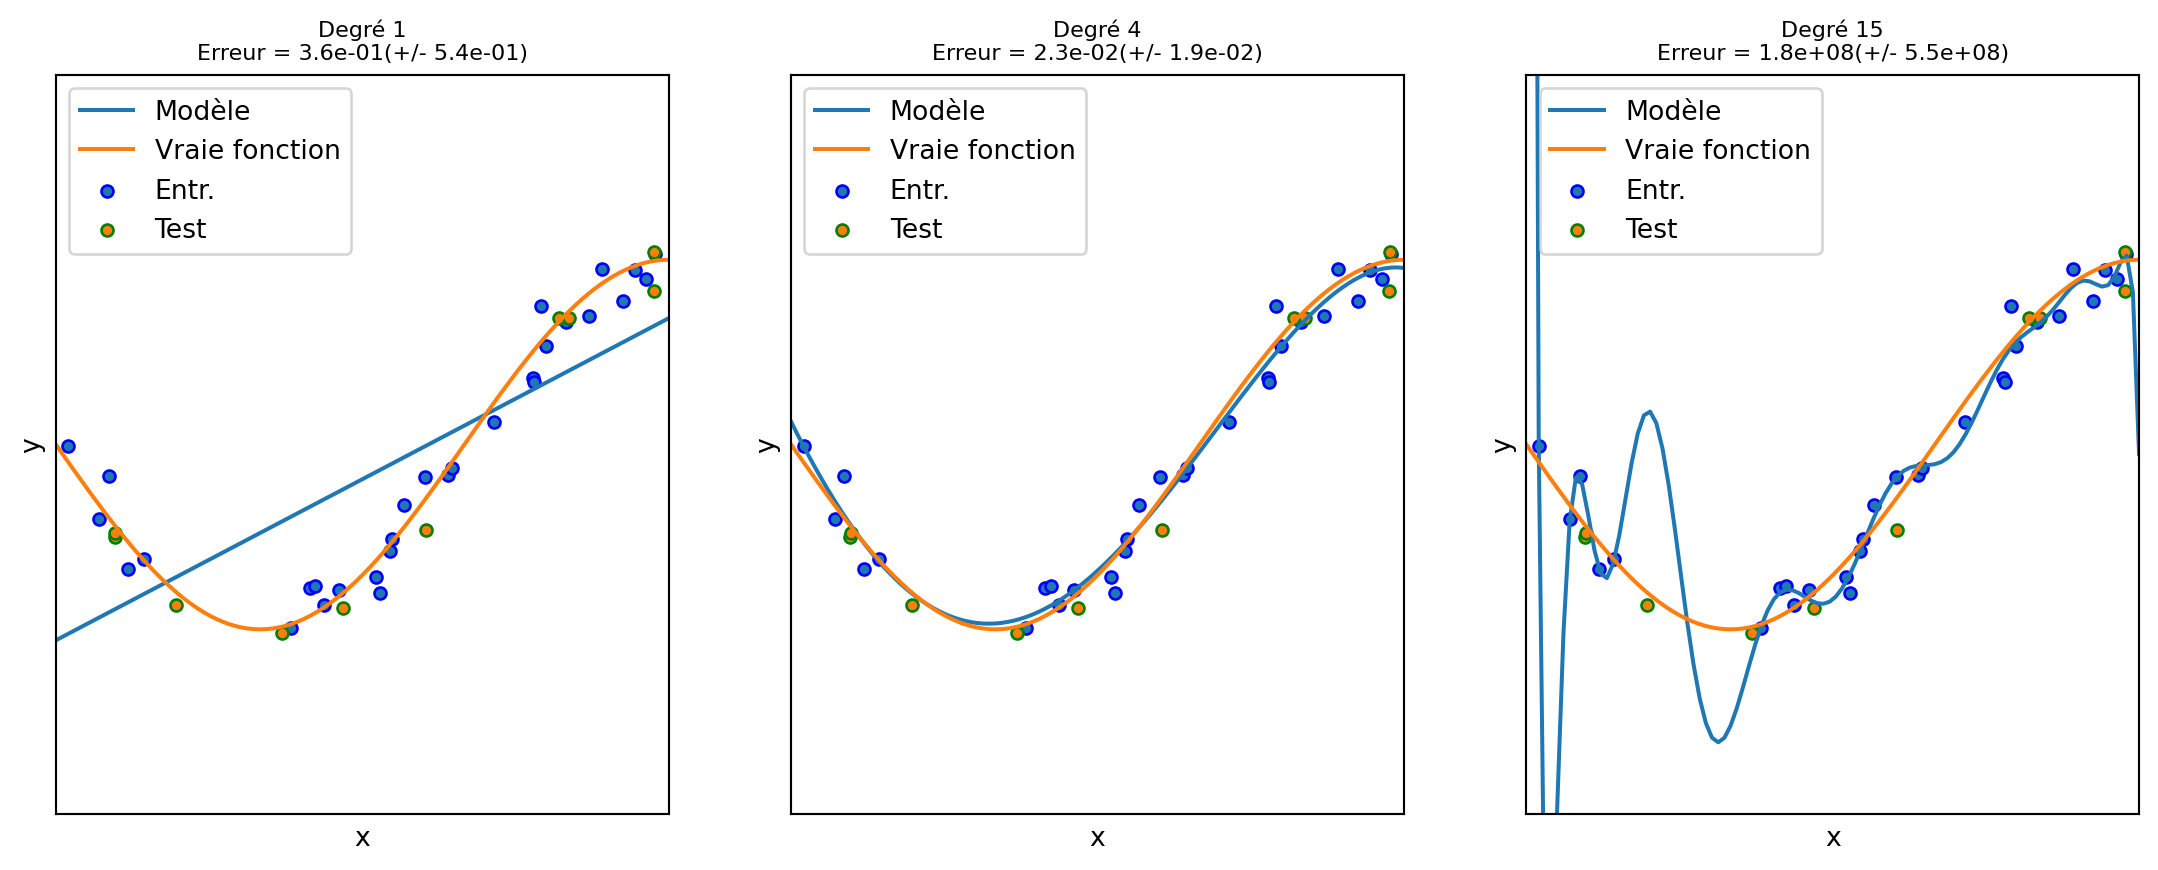
\includegraphics[width=11.23958in,height=4.53125in]{05-ClassificationsSupervisees_files/figure-html/fig-overfitting-output-1.png}
\caption{Figure~6.1: Exemples de sur et sous-apprentissage.}
\end{figure}

On constate aussi que sans les échantillons de validation, nous serions
incapable de déterminer la situation de sur-apprentissage, l'erreur sur
les points d'entraînement seul étant excellente pour un degré 15.

\subsubsection{\texorpdfstring{{6.2.2}
Pipeline}{6.2.2 Pipeline}}\label{pipeline}

La construction d'un modèle implique généralement toujours les mêmes
étapes illustrées sur la figure \hyperref[fig-pipeline]{figure~{6.2}}:

\begin{enumerate}
\def\labelenumi{\arabic{enumi}.}
\item
  La préparation des données implique parfois un pré-traitement afin de
  normaliser les données.
\item
  Partage des données en trois groupes: entraînement, validation et test
\item
  L'apprentissage du modèle sur l'ensemble d'entraînement. Cet
  apprentissage nécessite de déterminer les valeurs des hyper-paramètres
  du modèle par l'usager.
\item
  La validation du modèle sur l'ensemble de validation. Cette étape vise
  à vérifier que les hyper-paramètres du modèle sont adéquate.
\item
  Enfin le test du modèle sur un ensemble de donnée indépendant
\end{enumerate}

\phantomsection\label{fig-pipeline}
\begin{figure}
\centering
\begin{Shaded}
\begin{Highlighting}[]
\NormalTok{flowchart TD}
\NormalTok{    A[fa:fa{-}database Données] {-}{-}\textgreater{} B(fa:fa{-}gear Prétraitement)}
\NormalTok{    B {-}{-}\textgreater{} C(fa:fa{-}folder{-}tree Partage des données) {-}.{-}\textgreater{} D(fa:fa{-}gears Entraînement)}
\NormalTok{    H[[Hyper{-}paramètres]] {-}{-}\textgreater{} D}
\NormalTok{    D {-}{-}\textgreater{} |Modèle| E\textgreater{}Validation]}
\NormalTok{    E {-}{-}\textgreater{} |Modèle| G\textgreater{}Test]}
\NormalTok{    C {-}.{-}\textgreater{} E}
\NormalTok{    C {-}.{-}\textgreater{} G}
\end{Highlighting}
\end{Shaded}
\caption{Figure~6.2: Étapes standards dans un entraînement.}
\end{figure}

\phantomsection\label{sec-05.02.02}
\subsubsection{\texorpdfstring{{6.2.3} Construction d'un ensemble
d'entraînement}{6.2.3 Construction d'un ensemble d'entraînement}}\label{construction-dun-ensemble-dentrauxeenement}

Les données d'entraînement vont permettre de construire un modèle. Ces
données peuvent prendre des formes très variées mais on peut voir cela
sous la forme d'un tableau {\textbackslash(N \textbackslash times
D\textbackslash)}:

\begin{enumerate}
\def\labelenumi{\arabic{enumi}.}
\item
  La taille {\textbackslash(N\textbackslash)} du jeu de donnée
\item
  Chaque entrée définit un échantillon ou un point dans un espace à
  plusieurs dimension.
\item
  Chaque échantillon est décrit par {\textbackslash(D\textbackslash)}
  dimensions ou caractéristiques (\emph{features}).
\end{enumerate}

Une façon simple de construire un ensemble d'entraînement est
d'échantillonner un produit existant. Nous allons utiliser la carte
d'occupation des sols suivante qui contient 12 classes différentes.

\phantomsection\label{9edc7159}
\phantomsection\label{cb5}
\begin{Shaded}
\begin{Highlighting}[]
\NormalTok{couleurs\_classes}\OperatorTok{=}\NormalTok{ \{}\StringTok{\textquotesingle{}NoData\textquotesingle{}}\NormalTok{: }\StringTok{\textquotesingle{}black\textquotesingle{}}\NormalTok{, }\StringTok{\textquotesingle{}Commercial\textquotesingle{}}\NormalTok{: }\StringTok{\textquotesingle{}yellow\textquotesingle{}}\NormalTok{, }\StringTok{\textquotesingle{}Nuages\textquotesingle{}}\NormalTok{: }\StringTok{\textquotesingle{}lightgrey\textquotesingle{}}\NormalTok{, }
                    \StringTok{\textquotesingle{}Foret\textquotesingle{}}\NormalTok{: }\StringTok{\textquotesingle{}darkgreen\textquotesingle{}}\NormalTok{, }\StringTok{\textquotesingle{}Faible\_végétation\textquotesingle{}}\NormalTok{: }\StringTok{\textquotesingle{}green\textquotesingle{}}\NormalTok{, }\StringTok{\textquotesingle{}Sol\_nu\textquotesingle{}}\NormalTok{: }\StringTok{\textquotesingle{}saddlebrown\textquotesingle{}}\NormalTok{,}
                  \StringTok{\textquotesingle{}Roche\textquotesingle{}}\NormalTok{: }\StringTok{\textquotesingle{}dimgray\textquotesingle{}}\NormalTok{, }\StringTok{\textquotesingle{}Route\textquotesingle{}}\NormalTok{: }\StringTok{\textquotesingle{}red\textquotesingle{}}\NormalTok{, }\StringTok{\textquotesingle{}Urbain\textquotesingle{}}\NormalTok{: }\StringTok{\textquotesingle{}orange\textquotesingle{}}\NormalTok{, }\StringTok{\textquotesingle{}Eau\textquotesingle{}}\NormalTok{: }\StringTok{\textquotesingle{}blue\textquotesingle{}}\NormalTok{, }\StringTok{\textquotesingle{}Tourbe\textquotesingle{}}\NormalTok{: }\StringTok{\textquotesingle{}salmon\textquotesingle{}}\NormalTok{, }\StringTok{\textquotesingle{}Végétation éparse\textquotesingle{}}\NormalTok{: }\StringTok{\textquotesingle{}darkgoldenrod\textquotesingle{}}\NormalTok{, }\StringTok{\textquotesingle{}Roche avec végétation\textquotesingle{}}\NormalTok{: }\StringTok{\textquotesingle{}darkseagreen\textquotesingle{}}\NormalTok{\}}
\NormalTok{nom\_classes}\OperatorTok{=}\NormalTok{ [}\OperatorTok{*}\NormalTok{couleurs\_classes.keys()]}
\NormalTok{couleurs\_classes}\OperatorTok{=}\NormalTok{ [}\OperatorTok{*}\NormalTok{couleurs\_classes.values()]}
\end{Highlighting}
\end{Shaded}

On peut visualiser la carte de la façon suivante:

\phantomsection\label{5c61a76f}
\phantomsection\label{cb6}
\begin{Shaded}
\begin{Highlighting}[]
\ImportTok{import}\NormalTok{ matplotlib.pyplot }\ImportTok{as}\NormalTok{ plt}
\ImportTok{import}\NormalTok{ rioxarray }\ImportTok{as}\NormalTok{ rxr}
\NormalTok{cmap\_classes }\OperatorTok{=}\NormalTok{ ListedColormap(couleurs\_classes)}

\NormalTok{fig, ax }\OperatorTok{=}\NormalTok{ plt.subplots(nrows}\OperatorTok{=}\DecValTok{1}\NormalTok{, ncols}\OperatorTok{=}\DecValTok{1}\NormalTok{, figsize}\OperatorTok{=}\NormalTok{(}\DecValTok{8}\NormalTok{, }\DecValTok{6}\NormalTok{))}
\NormalTok{img\_carte.squeeze().plot.imshow(cmap}\OperatorTok{=}\NormalTok{cmap\_classes, vmin}\OperatorTok{=}\DecValTok{0}\NormalTok{, vmax}\OperatorTok{=}\DecValTok{12}\NormalTok{)}
\NormalTok{ax.set\_title(}\StringTok{"Carte d\textquotesingle{}occupation des sols"}\NormalTok{, fontsize}\OperatorTok{=}\StringTok{"small"}\NormalTok{)}
\end{Highlighting}
\end{Shaded}

\begin{verbatim}
Text(0.5, 1.0, "Carte d'occupation des sols")
\end{verbatim}

\begin{figure}
\centering
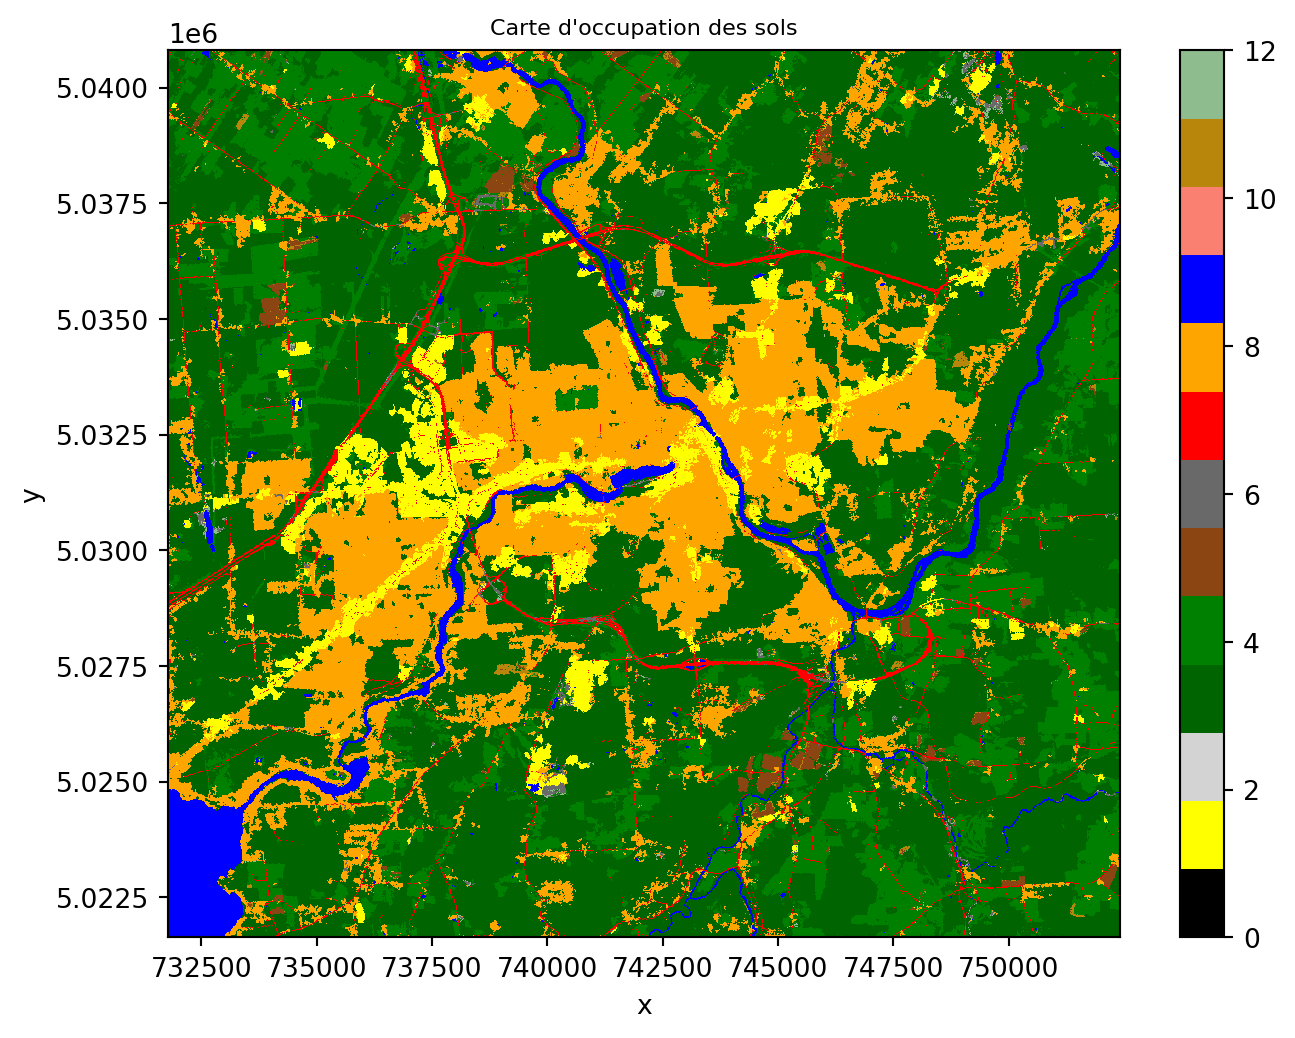
\includegraphics[width=6.75in,height=5.40625in]{05-ClassificationsSupervisees_files/figure-html/cell-8-output-2.png}
\caption{}
\end{figure}

On peut facilement calculer la fréquence d'occurrence des 12 classes
dans l'image à l'aide de \texttt{numpy}:

\phantomsection\label{8be8624a}
\phantomsection\label{cb8}
\begin{Shaded}
\begin{Highlighting}[]
\NormalTok{img\_carte}\OperatorTok{=}\NormalTok{ img\_carte.squeeze() }\CommentTok{\# nécessaire pour ignorer la dimension du canal}
\NormalTok{compte\_classe }\OperatorTok{=}\NormalTok{ np.unique(img\_carte.data, return\_counts}\OperatorTok{=}\VariableTok{True}\NormalTok{)}
\BuiltInTok{print}\NormalTok{(compte\_classe)}
\end{Highlighting}
\end{Shaded}

\begin{verbatim}
(array([ 1.,  3.,  4.,  5.,  6.,  7.,  8.,  9., 11., 12., nan],
      dtype=float32), array([ 193558, 2104777,  670158,   29523,   14624,   94751,  750046,
        123671,    9079,    4327,      10]))
\end{verbatim}

La fréquence d'apparition de chaque classe varie grandement, on parle
alors d'un \textbf{ensemble déséquilibré}. Ceci est très commun dans la
plupart des ensembles d'entraînement, les classes n'apparaissent pas
avec la même fréquence.

\phantomsection\label{adfdd31d}
\phantomsection\label{cb10}
\begin{Shaded}
\begin{Highlighting}[]
\NormalTok{valeurs, comptes }\OperatorTok{=}\NormalTok{ compte\_classe}

\CommentTok{\# Create the histogram}
\NormalTok{plt.figure(figsize}\OperatorTok{=}\NormalTok{(}\DecValTok{5}\NormalTok{, }\DecValTok{3}\NormalTok{))}
\NormalTok{plt.bar(valeurs, comptes}\OperatorTok{/}\NormalTok{comptes.}\BuiltInTok{sum}\NormalTok{()}\OperatorTok{*}\DecValTok{100}\NormalTok{)}
\NormalTok{plt.xlabel(}\StringTok{"Classes"}\NormalTok{)}
\NormalTok{plt.ylabel(}\StringTok{"\%"}\NormalTok{)}
\NormalTok{plt.title(}\StringTok{"Fréquences des classes"}\NormalTok{, fontsize}\OperatorTok{=}\StringTok{"small"}\NormalTok{)}
\NormalTok{plt.xticks(}\BuiltInTok{range}\NormalTok{(}\BuiltInTok{len}\NormalTok{(nom\_classes)), nom\_classes, rotation}\OperatorTok{=}\DecValTok{45}\NormalTok{, ha}\OperatorTok{=}\StringTok{\textquotesingle{}right\textquotesingle{}}\NormalTok{)}
\NormalTok{plt.show()}
\end{Highlighting}
\end{Shaded}

\begin{figure}
\centering
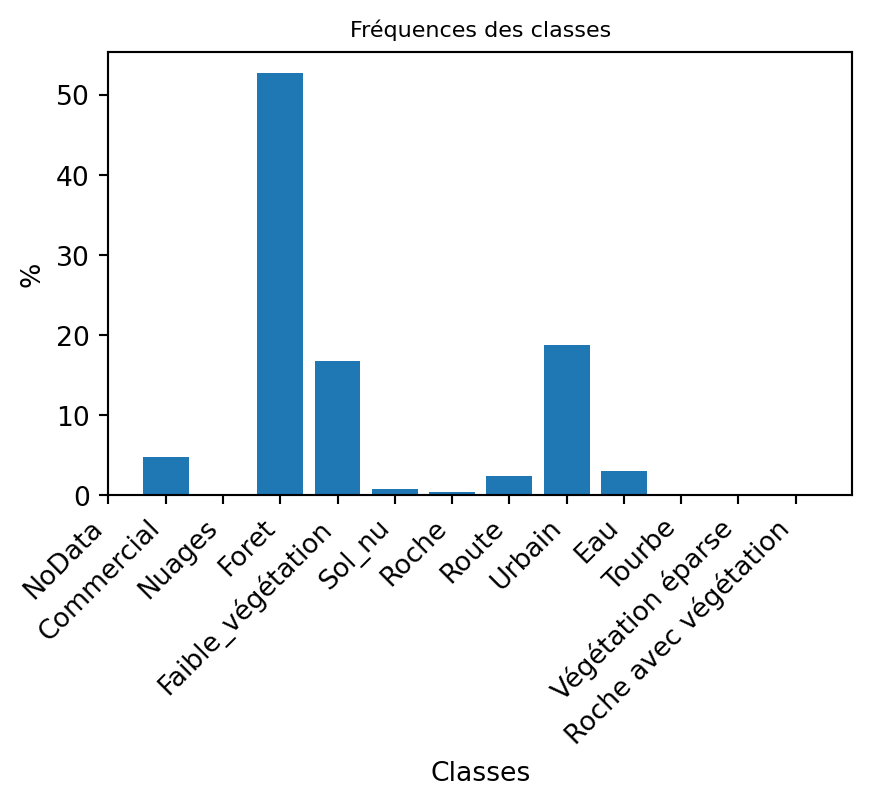
\includegraphics[width=4.54167in,height=4.19792in]{05-ClassificationsSupervisees_files/figure-html/cell-10-output-1.png}
\caption{}
\end{figure}

On peut échantillonner 100 points aléatoires pour chaque classe:

\phantomsection\label{a061c0ea}
\phantomsection\label{cb11}
\begin{Shaded}
\begin{Highlighting}[]
\NormalTok{img\_carte}\OperatorTok{=}\NormalTok{ img\_carte.squeeze()}
\NormalTok{class\_counts }\OperatorTok{=}\NormalTok{ np.unique(img\_carte.data, return\_counts}\OperatorTok{=}\VariableTok{True}\NormalTok{)}

\CommentTok{\# Liste vide des points échantillonnées}
\NormalTok{sampled\_points }\OperatorTok{=}\NormalTok{ []}
\NormalTok{class\_labels}\OperatorTok{=}\NormalTok{ [] }\CommentTok{\# contient les étiquettes des classes}
\ControlFlowTok{for}\NormalTok{ class\_label }\KeywordTok{in} \BuiltInTok{range}\NormalTok{(}\DecValTok{1}\NormalTok{,}\DecValTok{13}\NormalTok{): }\CommentTok{\# pour chacune des 12 classes}
  \CommentTok{\# On cherche tous les pixels pour cette étiquette}
\NormalTok{  class\_pixels }\OperatorTok{=}\NormalTok{ np.argwhere(img\_carte.data }\OperatorTok{==}\NormalTok{ class\_label)}

  \CommentTok{\# On se limite à 100 pixels par classe}
\NormalTok{  n\_samples }\OperatorTok{=} \BuiltInTok{min}\NormalTok{(}\DecValTok{100}\NormalTok{, }\BuiltInTok{len}\NormalTok{(class\_pixels))}

  \CommentTok{\# On les choisit les positions aléatoirement}
\NormalTok{  np.random.seed(}\DecValTok{0}\NormalTok{) }\CommentTok{\# ceci permet de répliquer le tirage aléatoire}
\NormalTok{  sampled\_indices }\OperatorTok{=}\NormalTok{ np.random.choice(}\BuiltInTok{len}\NormalTok{(class\_pixels), n\_samples, replace}\OperatorTok{=}\VariableTok{False}\NormalTok{)}

  \CommentTok{\# On prends les positions en lignes, colonnes}
\NormalTok{  sampled\_pixels }\OperatorTok{=}\NormalTok{ class\_pixels[sampled\_indices]}

  \CommentTok{\# On ajoute les points à la liste}
\NormalTok{  sampled\_points.extend(sampled\_pixels)}
\NormalTok{  class\_labels.extend(np.array([class\_label]}\OperatorTok{*}\NormalTok{n\_samples)[:,np.newaxis])}

\CommentTok{\# Conversion en NumPy array}
\NormalTok{sampled\_points }\OperatorTok{=}\NormalTok{ np.array(sampled\_points)}
\NormalTok{class\_labels }\OperatorTok{=}\NormalTok{ np.array(class\_labels)}
\CommentTok{\# On peut naviguer les points à l\textquotesingle{}aide de la géoréférence}
\NormalTok{transformer }\OperatorTok{=}\NormalTok{ rasterio.transform.AffineTransformer(img\_carte.rio.transform())}
\NormalTok{transform\_sampled\_points}\OperatorTok{=}\NormalTok{ transformer.xy(sampled\_points[:,}\DecValTok{0}\NormalTok{], sampled\_points[:,}\DecValTok{1}\NormalTok{])}

\NormalTok{fig, ax }\OperatorTok{=}\NormalTok{ plt.subplots(nrows}\OperatorTok{=}\DecValTok{1}\NormalTok{, ncols}\OperatorTok{=}\DecValTok{1}\NormalTok{, figsize}\OperatorTok{=}\NormalTok{(}\DecValTok{8}\NormalTok{, }\DecValTok{6}\NormalTok{))}
\NormalTok{img\_carte.squeeze().plot.imshow(cmap}\OperatorTok{=}\NormalTok{cmap\_classes, vmin}\OperatorTok{=}\DecValTok{0}\NormalTok{, vmax}\OperatorTok{=}\DecValTok{12}\NormalTok{)}
\NormalTok{ax.scatter(transform\_sampled\_points[}\DecValTok{0}\NormalTok{], transform\_sampled\_points[}\DecValTok{1}\NormalTok{], c}\OperatorTok{=}\StringTok{\textquotesingle{}w\textquotesingle{}}\NormalTok{, s}\OperatorTok{=}\DecValTok{1}\NormalTok{)  }\CommentTok{\# Plot sampled points}
\NormalTok{ax.set\_title(}\StringTok{"Carte d\textquotesingle{}occupation des sols avec les points échantillonnés"}\NormalTok{, fontsize}\OperatorTok{=}\StringTok{"small"}\NormalTok{)}
\NormalTok{plt.show()}
\end{Highlighting}
\end{Shaded}

\begin{figure}
\centering
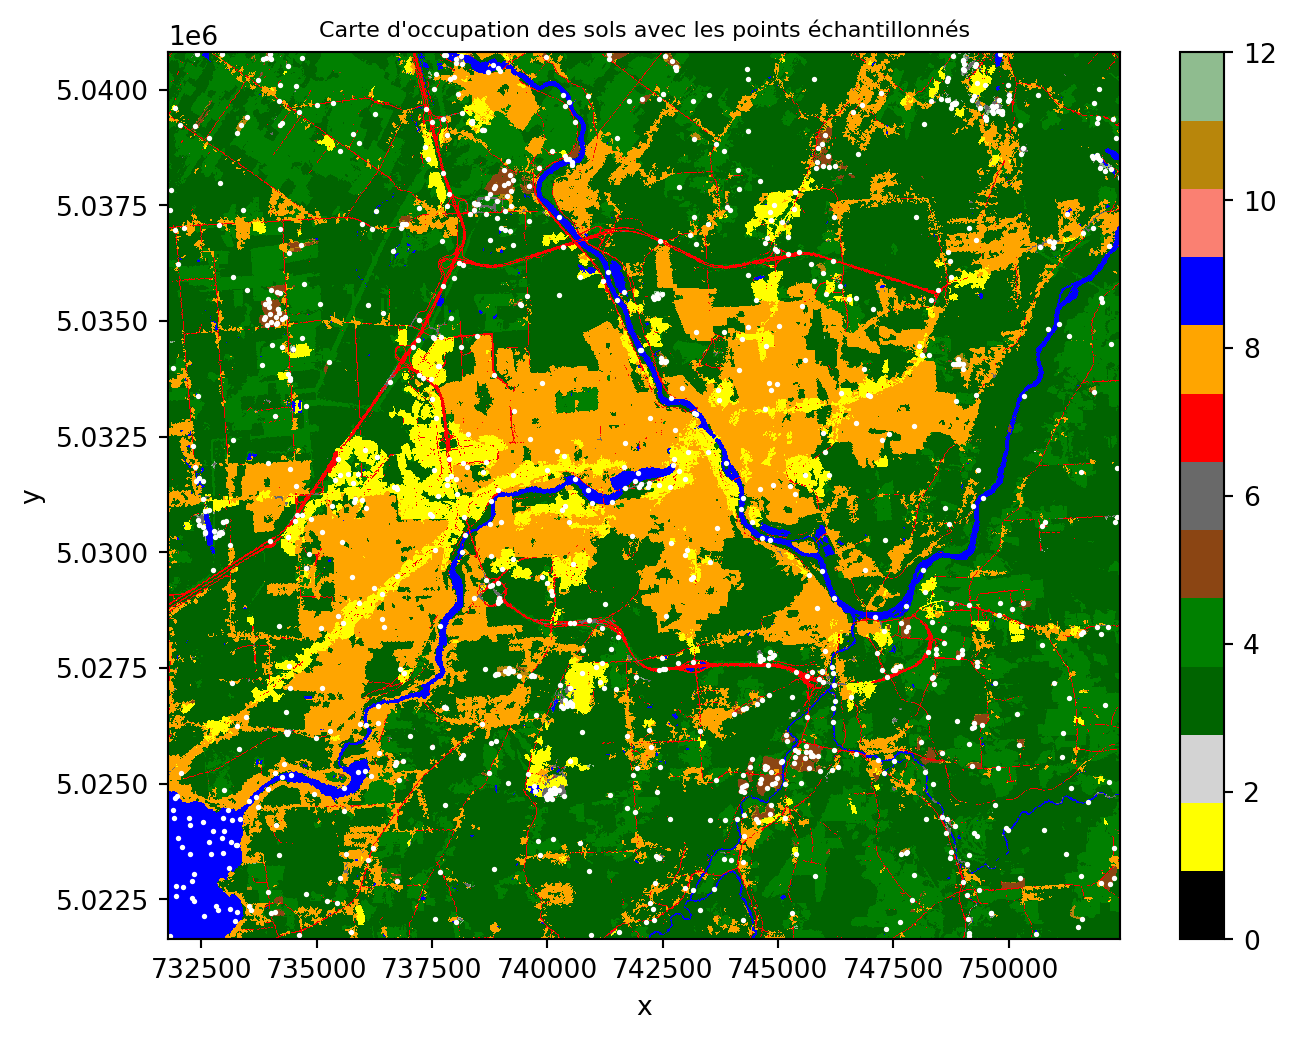
\includegraphics[width=6.75in,height=5.41667in]{05-ClassificationsSupervisees_files/figure-html/cell-11-output-1.png}
\caption{}
\end{figure}

Une fois les points sélectionnés, il faut ajouter les valeurs des bandes
provenant d'une image satellite. Pour cela, on peut utiliser la méthodes
\texttt{sample()} de \texttt{rasterio}. Éventuellement, la librairie
\href{https://geopandas.org}{\texttt{geopandas}} permet de gérer les
données d'entraînement sous la forme d'un tableau transportant aussi
l'information de géoréférence. Afin de pouvoir classifier ces points,
nous allons ajouter les valeurs radiométriques provenant de l'image
Sentinel-2 à 4 bandes \texttt{RGBNIR\_of\_S2A.tif}. Ces valeurs seront
stockées dans la colonne \texttt{value} sous la forme d'un vecteur en
format \texttt{string}:

\phantomsection\label{4b62cf70}
\phantomsection\label{cb12}
\begin{Shaded}
\begin{Highlighting}[]
\NormalTok{points }\OperatorTok{=}\NormalTok{ [Point(xy) }\ControlFlowTok{for}\NormalTok{ xy }\KeywordTok{in} \BuiltInTok{zip}\NormalTok{(transform\_sampled\_points[}\DecValTok{0}\NormalTok{], transform\_sampled\_points[}\DecValTok{1}\NormalTok{])]}
\NormalTok{gdf }\OperatorTok{=}\NormalTok{ geopandas.GeoDataFrame(}\BuiltInTok{range}\NormalTok{(}\DecValTok{1}\NormalTok{,}\BuiltInTok{len}\NormalTok{(points)}\OperatorTok{+}\DecValTok{1}\NormalTok{), geometry}\OperatorTok{=}\NormalTok{points, crs}\OperatorTok{=}\NormalTok{img\_carte.rio.crs)}
\NormalTok{coord\_list }\OperatorTok{=}\NormalTok{ [(x, y) }\ControlFlowTok{for}\NormalTok{ x, y }\KeywordTok{in} \BuiltInTok{zip}\NormalTok{(gdf[}\StringTok{"geometry"}\NormalTok{].x, gdf[}\StringTok{"geometry"}\NormalTok{].y)]}
\ControlFlowTok{with}\NormalTok{ rasterio.}\BuiltInTok{open}\NormalTok{(}\StringTok{\textquotesingle{}RGBNIR\_of\_S2A.tif\textquotesingle{}}\NormalTok{) }\ImportTok{as}\NormalTok{ src:}
\NormalTok{  gdf[}\StringTok{"value"}\NormalTok{] }\OperatorTok{=}\NormalTok{ [x }\ControlFlowTok{for}\NormalTok{ x }\KeywordTok{in}\NormalTok{ src.sample(coord\_list)]}
\NormalTok{gdf[}\StringTok{\textquotesingle{}class\textquotesingle{}}\NormalTok{]}\OperatorTok{=}\NormalTok{ class\_labels}
\NormalTok{gdf.to\_csv(}\StringTok{\textquotesingle{}sampling\_points.csv\textquotesingle{}}\NormalTok{) }\CommentTok{\# sauvegarde sous forme d\textquotesingle{}un format csv}
\NormalTok{gdf.head()}
\end{Highlighting}
\end{Shaded}

\begin{longtable}[]{@{}lllll@{}}
\toprule\noalign{}
& 0 & geometry & value & class \\
\midrule\noalign{}
\endhead
\bottomrule\noalign{}
\endlastfoot
0 & 1 & POINT (740369.77 5032078.683) & {[}1894, 1994, 2112, 2318{]} &
1 \\
1 & 2 & POINT (737542.924 5031770.119) & {[}1440, 1650, 1449, 5021{]} &
1 \\
2 & 3 & POINT (736726.722 5031411.786) & {[}1666, 1972, 1819, 3437{]} &
1 \\
3 & 4 & POINT (736816.305 5027470.128) & {[}1858, 2078, 2190, 2436{]} &
1 \\
4 & 5 & POINT (736746.629 5031362.018) & {[}2194, 2304, 2268, 3075{]} &
1 \\
\end{longtable}

\subsection{\texorpdfstring{{6.3} Analyse préliminaire des
données}{6.3 Analyse préliminaire des données}}\label{analyse-pruxe9liminaire-des-donnuxe9es}

Une bonne pratique avant d'appliquer une technique d'apprentissage
automatique est de regarder les caractéristiques de vos données:

\begin{enumerate}
\def\labelenumi{\arabic{enumi}.}
\item
  Le nombre de dimensions (\emph{features})
\item
  Certaines dimensions sont informatives (discriminantes) et d'autres ne
  le sont pas
\item
  Le nombre classes
\item
  Le nombre de modes (\emph{clusters}) par classes
\item
  Le nombre d'échantillons par classe
\item
  La forme des groupes
\item
  La séparabilité des classes ou des groupes
\end{enumerate}

Une manière d'évaluer la séparabilité de vos classes est d'appliquer des
modèles Gaussiens sur chacune des classes. Le modèle Gaussien multivarié
suppose que les données sont distribuées comme un nuage de points
symétrique et unimodale. La distribution d'un point
{\textbackslash(x\textbackslash)} appartenant à la classe
{\textbackslash(i\textbackslash)} est la suivante:

{\textbackslash{[} P(x \textbar{} Classe=i) =
\textbackslash frac\{1\}\{(2\textbackslash pi)\^{}\{D/2\}
\textbar\textbackslash Sigma\_i\textbar\^{}\{1/2\}\}\textbackslash exp\textbackslash left(-\textbackslash frac\{1\}\{2\}
(x-m\_i)\^{}t \textbackslash Sigma\_k\^{}\{-1\}
(x-m\_i)\textbackslash right) \textbackslash{]}}

La méthode
\href{https://scikit-learn.org/stable/modules/generated/sklearn.discriminant_analysis.QuadraticDiscriminantAnalysis.html}{\texttt{QuadraticDiscriminantAnalysis}}
permet de calculer les paramètres des Gaussiennes multivariées pour
chacune des classes.

On peut calculer une distance entre deux nuages Gaussiens avec la
distance dites de Jeffries-Matusita (JM) basée sur la distance de
Bhattacharyya {\textbackslash(B\textbackslash)}:

{\textbackslash{[} JM\_\{ij\}=
2(1-e\^{}\{-B\})\textbackslash\textbackslash{}
B=\textbackslash frac\{1\}\{8\}(m\_i-m\_j)\^{}t \{
\textbackslash frac\{\textbackslash Sigma\_i+\textbackslash Sigma\_j\}\{2\}
\}(m\_i-m\_j)+\textbackslash frac\{1\}\{2\}ln \{
\textbackslash frac\{\textbar(\textbackslash Sigma\_i+\textbackslash Sigma\_j)/2\textbar\}\{\textbar\textbackslash Sigma\_i\textbar\^{}\{1/2\}\textbar\textbackslash Sigma\_j\textbar\^{}\{1/2\}\}\}
\textbackslash{]}}

Cette distance présuppose que chaque classe
{\textbackslash(i\textbackslash)} est décrite par son centre
{\textbackslash(m\_i\textbackslash)} et de sa dispersion dans l'espace à
{\textbackslash(D\textbackslash)} dimensions mesurée par la matrice de
covariance {\textbackslash(\textbackslash Sigma\_i\textbackslash)}. On
peut en faire facilement une fonction Python à l'aide de \texttt{numpy}:

\phantomsection\label{dda7b492}
\phantomsection\label{cb13}
\begin{Shaded}
\begin{Highlighting}[]
\KeywordTok{def}\NormalTok{ bhattacharyya\_distance(m1, s1, m2, s2):}
    \CommentTok{\# Calcul de la covariance moyenne}
\NormalTok{    s }\OperatorTok{=}\NormalTok{ (s1 }\OperatorTok{+}\NormalTok{ s2) }\OperatorTok{/} \DecValTok{2}
    
    \CommentTok{\# Calcul du premier terme (différence des moyennes)}
\NormalTok{    m\_diff }\OperatorTok{=}\NormalTok{ m1 }\OperatorTok{{-}}\NormalTok{ m2}
\NormalTok{    term1 }\OperatorTok{=}\NormalTok{ np.dot(np.dot(m\_diff.T, np.linalg.inv(s)), m\_diff) }\OperatorTok{/} \DecValTok{8}
    
    \CommentTok{\# Calcul du second terme (différence de covariances)}
\NormalTok{    term2 }\OperatorTok{=} \FloatTok{0.5} \OperatorTok{*}\NormalTok{ np.log(np.linalg.det(s) }\OperatorTok{/}\NormalTok{ np.sqrt(np.linalg.det(s1) }\OperatorTok{*}\NormalTok{ np.linalg.det(s2)))}
    
    \ControlFlowTok{return}\NormalTok{ term1 }\OperatorTok{+}\NormalTok{ term2}

\KeywordTok{def}\NormalTok{ jeffries\_matusita\_distance(m1, s1, m2, s2):}
\NormalTok{    B }\OperatorTok{=}\NormalTok{ bhattacharyya\_distance(m1, s1, m2, s2)}
    \ControlFlowTok{return} \DecValTok{2} \OperatorTok{*}\NormalTok{ (}\DecValTok{1} \OperatorTok{{-}}\NormalTok{ np.exp(}\OperatorTok{{-}}\NormalTok{B))}
\end{Highlighting}
\end{Shaded}

La figure ci-dessous illustre différentes situations avec des données
artificielles:

\phantomsection\label{1c13f01b}
\begin{figure}
\centering
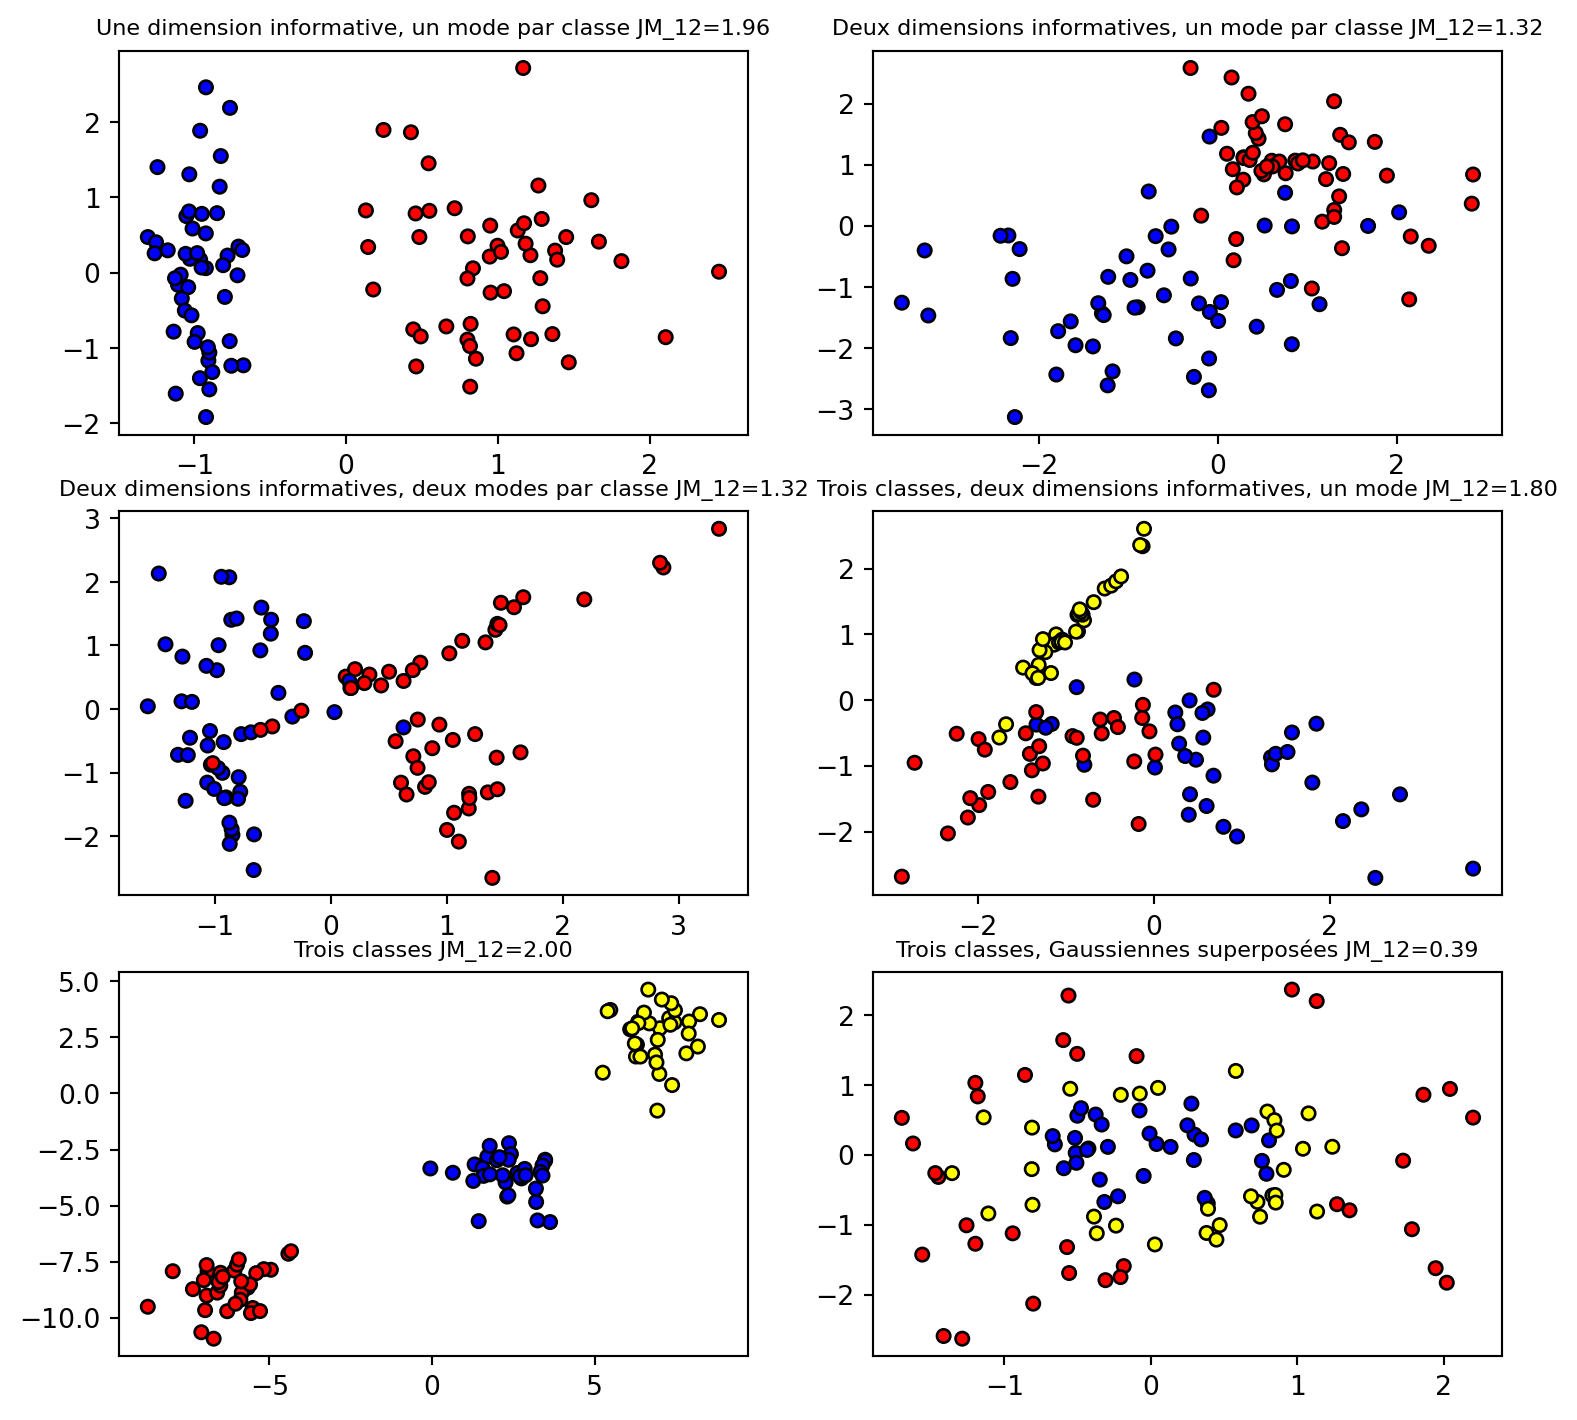
\includegraphics[width=8.21875in,height=7.39583in]{05-ClassificationsSupervisees_files/figure-html/cell-14-output-1.png}
\caption{}
\end{figure}

On forme notre ensemble d'entrainement à partir du fichier \texttt{csv}
de la section \hyperref[sec-05.02.02]{{Section 6.2.3}}.

\phantomsection\label{203f61c8}
\phantomsection\label{cb14}
\begin{Shaded}
\begin{Highlighting}[]
\NormalTok{df}\OperatorTok{=}\NormalTok{ pd.read\_csv(}\StringTok{\textquotesingle{}sampling\_points.csv\textquotesingle{}}\NormalTok{)}
\CommentTok{\# Extraire la colonne \textquotesingle{}value\textquotesingle{}.}
\CommentTok{\# \textquotesingle{}value\textquotesingle{} est une chaîne de caractères représentation d\textquotesingle{}une liste de nombres.}
\CommentTok{\# Nous devons la convertir en données numériques réelles.}
\NormalTok{X }\OperatorTok{=}\NormalTok{ df[}\StringTok{\textquotesingle{}value\textquotesingle{}}\NormalTok{].}\BuiltInTok{apply}\NormalTok{(}\KeywordTok{lambda}\NormalTok{ x: np.fromstring(x[}\DecValTok{1}\NormalTok{:}\OperatorTok{{-}}\DecValTok{1}\NormalTok{], dtype}\OperatorTok{=}\BuiltInTok{float}\NormalTok{, sep}\OperatorTok{=}\StringTok{\textquotesingle{} \textquotesingle{}}\NormalTok{)).to\_list()}

\CommentTok{\# on obtient une liste de numpy array  qu\textquotesingle{}il faut convertir en un numpy array 2D}
\NormalTok{X}\OperatorTok{=}\NormalTok{ np.array([row.tolist() }\ControlFlowTok{for}\NormalTok{ row }\KeywordTok{in}\NormalTok{ X])}
\NormalTok{idx}\OperatorTok{=}\NormalTok{ X.}\BuiltInTok{sum}\NormalTok{(axis}\OperatorTok{={-}}\DecValTok{1}\NormalTok{)}\OperatorTok{\textgreater{}}\DecValTok{0} \CommentTok{\# on exclut certains points sans valeurs}
\NormalTok{X}\OperatorTok{=}\NormalTok{ X[idx,...]}
\NormalTok{y }\OperatorTok{=}\NormalTok{ df[}\StringTok{\textquotesingle{}class\textquotesingle{}}\NormalTok{].to\_numpy()}
\NormalTok{y}\OperatorTok{=}\NormalTok{ y[idx]}
\NormalTok{class\_labels }\OperatorTok{=}\NormalTok{ np.unique(y).tolist() }\CommentTok{\# on cherche à savoir combien de classes uniques}
\NormalTok{n\_classes }\OperatorTok{=} \BuiltInTok{len}\NormalTok{(class\_labels)}
\ControlFlowTok{if} \BuiltInTok{max}\NormalTok{(class\_labels) }\OperatorTok{\textgreater{}}\NormalTok{ n\_classes: }\CommentTok{\# il se peut que certaines classes soit absentes}
\NormalTok{  y\_new}\OperatorTok{=}\NormalTok{ []}
  \ControlFlowTok{for}\NormalTok{ i,l }\KeywordTok{in} \BuiltInTok{enumerate}\NormalTok{(class\_labels):}
\NormalTok{    y\_new.extend([i]}\OperatorTok{*}\BuiltInTok{sum}\NormalTok{(y}\OperatorTok{==}\NormalTok{l))}
\NormalTok{  y\_new }\OperatorTok{=}\NormalTok{ np.array(y\_new)}

\NormalTok{couleurs\_classes2}\OperatorTok{=}\NormalTok{ [couleurs\_classes[c] }\ControlFlowTok{for}\NormalTok{ c }\KeywordTok{in}\NormalTok{ np.unique(y).tolist()] }\CommentTok{\# couleurs des classes}
\NormalTok{nom\_classes2}\OperatorTok{=}\NormalTok{ [nom\_classes[c] }\ControlFlowTok{for}\NormalTok{ c }\KeywordTok{in}\NormalTok{ np.unique(y).tolist()]}
\NormalTok{cmap\_classes2 }\OperatorTok{=}\NormalTok{ ListedColormap(couleurs\_classes2)}
\end{Highlighting}
\end{Shaded}

On peut faire une analyse de séparabilité sur notre ensemble
d'entrainement de 10 classes. On obtient un tableau symmétrique de 10x10
valeurs. On peut observer des valeurs inférieures à 1 ce qui indique des
séparabilités faibles entre ces classes sous l'hypothèse du modèle
Gaussien:

\phantomsection\label{16c78db6}
\phantomsection\label{cb15}
\begin{Shaded}
\begin{Highlighting}[]
\NormalTok{qda}\OperatorTok{=}\NormalTok{ QuadraticDiscriminantAnalysis(store\_covariance}\OperatorTok{=}\VariableTok{True}\NormalTok{)}
\NormalTok{qda.fit(X, y\_new) }\CommentTok{\# calcul des paramètres des distributions Gaussiennes}
\NormalTok{JM}\OperatorTok{=}\NormalTok{ []}
\NormalTok{classes}\OperatorTok{=}\NormalTok{ np.unique(y\_new).tolist() }\CommentTok{\# étiquettes uniques des classes}
\ControlFlowTok{for}\NormalTok{ cl1 }\KeywordTok{in}\NormalTok{ classes:}
  \ControlFlowTok{for}\NormalTok{ cl2 }\KeywordTok{in}\NormalTok{ classes:}
\NormalTok{    JM.append(jeffries\_matusita\_distance(qda.means\_[cl1], qda.covariance\_[cl1], qda.means\_[cl2], qda.covariance\_[cl2]))}

\NormalTok{JM}\OperatorTok{=}\NormalTok{ np.array(JM).reshape(}\BuiltInTok{len}\NormalTok{(classes),}\BuiltInTok{len}\NormalTok{(classes))}
\NormalTok{JM}\OperatorTok{=}\NormalTok{ pd.DataFrame(JM, index}\OperatorTok{=}\NormalTok{classes, columns}\OperatorTok{=}\NormalTok{classes)}
\NormalTok{JM.head(}\DecValTok{10}\NormalTok{)}
\end{Highlighting}
\end{Shaded}

\begin{longtable}[]{@{}lllllllllll@{}}
\toprule\noalign{}
& 0 & 1 & 2 & 3 & 4 & 5 & 6 & 7 & 8 & 9 \\
\midrule\noalign{}
\endhead
\bottomrule\noalign{}
\endlastfoot
0 & 0.000000 & 1.931891 & 1.809590 & 1.761760 & 1.156486 & 1.326107 &
1.319344 & 1.830671 & 1.873676 & 1.700417 \\
1 & 1.931891 & 0.000000 & 1.082978 & 0.918865 & 1.788737 & 1.527192 &
1.331400 & 1.901749 & 0.854802 & 1.133180 \\
2 & 1.809590 & 1.082978 & 0.000000 & 0.266647 & 1.428062 & 1.255001 &
1.198888 & 1.947302 & 0.193032 & 0.782982 \\
3 & 1.761760 & 0.918865 & 0.266647 & 0.000000 & 1.413401 & 1.219793 &
1.127950 & 1.929637 & 0.377379 & 0.840250 \\
4 & 1.156486 & 1.788737 & 1.428062 & 1.413401 & 0.000000 & 0.397103 &
0.596618 & 1.956182 & 1.517926 & 1.036828 \\
5 & 1.326107 & 1.527192 & 1.255001 & 1.219793 & 0.397103 & 0.000000 &
0.167221 & 1.976696 & 1.248383 & 0.660213 \\
6 & 1.319344 & 1.331400 & 1.198888 & 1.127950 & 0.596618 & 0.167221 &
0.000000 & 1.956804 & 1.207618 & 0.660589 \\
7 & 1.830671 & 1.901749 & 1.947302 & 1.929637 & 1.956182 & 1.976696 &
1.956804 & 0.000000 & 1.966022 & 1.886064 \\
8 & 1.873676 & 0.854802 & 0.193032 & 0.377379 & 1.517926 & 1.248383 &
1.207618 & 1.966022 & 0.000000 & 0.741273 \\
9 & 1.700417 & 1.133180 & 0.782982 & 0.840250 & 1.036828 & 0.660213 &
0.660589 & 1.886064 & 0.741273 & 0.000000 \\
\end{longtable}

Afin d'évaluer chaque classe, on peut calculer la séparabilité minimale,
on peut observer que la classe eau a le maximum de séparabilité avec les
autres classes.

\phantomsection\label{f8b38b5a}
\begin{figure}
\centering
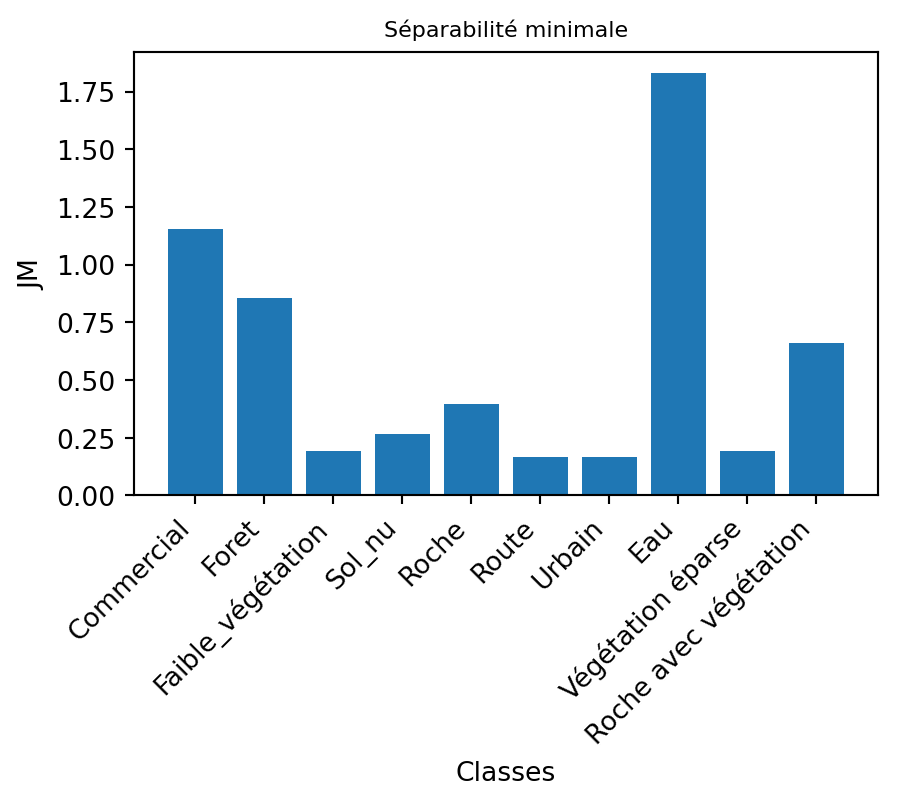
\includegraphics[width=4.67708in,height=4.19792in]{05-ClassificationsSupervisees_files/figure-html/cell-17-output-1.png}
\caption{}
\end{figure}

\subsection{\texorpdfstring{{6.4} Mesures de performance d'une méthode
de
classification}{6.4 Mesures de performance d'une méthode de classification}}\label{mesures-de-performance-dune-muxe9thode-de-classification}

Lorsque que l'on cherche à établir la performance d'un modèle, il faut
être capable de mesurer la performance de ce classificateur. Il existe
de nombreuses mesures de performance qui sont toutes dérivées de la
matrice de confusion. Cette matrice compare les étiquettes provenant de
l'annotation (la vérité terrain) et les étiquettes prédites par un
modèle. On peut définir {\textbackslash(C(i,j)\textbackslash)} est le
nombre de prédictions dont la vérité terrain indique la classe
{\textbackslash(i\textbackslash)} et qui sont prédites dans la classe
{\textbackslash(j\textbackslash)}. La fonction
\href{https://scikit-learn.org/stable/modules/generated/sklearn.metrics.confusion_matrix.html}{confusion\_matrix}
permet de faire ce calcul, voici un exemple très simple:

\phantomsection\label{dd534953}
\phantomsection\label{cb16}
\begin{Shaded}
\begin{Highlighting}[]
\NormalTok{y\_true }\OperatorTok{=}\NormalTok{ [}\StringTok{"cat"}\NormalTok{, }\StringTok{"ant"}\NormalTok{, }\StringTok{"cat"}\NormalTok{, }\StringTok{"cat"}\NormalTok{, }\StringTok{"ant"}\NormalTok{, }\StringTok{"bird"}\NormalTok{, }\StringTok{"bird"}\NormalTok{]}
\NormalTok{y\_pred }\OperatorTok{=}\NormalTok{ [}\StringTok{"ant"}\NormalTok{, }\StringTok{"ant"}\NormalTok{, }\StringTok{"cat"}\NormalTok{, }\StringTok{"cat"}\NormalTok{, }\StringTok{"ant"}\NormalTok{, }\StringTok{"cat"}\NormalTok{, }\StringTok{"bird"}\NormalTok{]}
\NormalTok{confusion\_matrix(y\_true, y\_pred, labels}\OperatorTok{=}\NormalTok{[}\StringTok{"ant"}\NormalTok{, }\StringTok{"bird"}\NormalTok{, }\StringTok{"cat"}\NormalTok{])}
\end{Highlighting}
\end{Shaded}

\begin{verbatim}
array([[2, 0, 0],
       [0, 1, 1],
       [1, 0, 2]])
\end{verbatim}

La fonction
\href{https://scikit-learn.org/stable/modules/generated/sklearn.metrics.classification_report.html\#sklearn.metrics.classification_report}{classification\_report}
permet de générer quelques métriques:

\phantomsection\label{c4b26260}
\phantomsection\label{cb18}
\begin{Shaded}
\begin{Highlighting}[]
\NormalTok{y\_true }\OperatorTok{=}\NormalTok{ [}\StringTok{"cat"}\NormalTok{, }\StringTok{"ant"}\NormalTok{, }\StringTok{"cat"}\NormalTok{, }\StringTok{"cat"}\NormalTok{, }\StringTok{"ant"}\NormalTok{, }\StringTok{"bird"}\NormalTok{, }\StringTok{"bird"}\NormalTok{]}
\NormalTok{y\_pred }\OperatorTok{=}\NormalTok{ [}\StringTok{"ant"}\NormalTok{, }\StringTok{"ant"}\NormalTok{, }\StringTok{"cat"}\NormalTok{, }\StringTok{"cat"}\NormalTok{, }\StringTok{"ant"}\NormalTok{, }\StringTok{"cat"}\NormalTok{, }\StringTok{"bird"}\NormalTok{]}
\BuiltInTok{print}\NormalTok{(classification\_report(y\_true, y\_pred, target\_names}\OperatorTok{=}\NormalTok{[}\StringTok{"ant"}\NormalTok{, }\StringTok{"bird"}\NormalTok{, }\StringTok{"cat"}\NormalTok{]))}
\end{Highlighting}
\end{Shaded}

\begin{verbatim}
              precision    recall  f1-score   support

         ant       0.67      1.00      0.80         2
        bird       1.00      0.50      0.67         2
         cat       0.67      0.67      0.67         3

    accuracy                           0.71         7
   macro avg       0.78      0.72      0.71         7
weighted avg       0.76      0.71      0.70         7
\end{verbatim}

Le rappel (\emph{recall}) pour une classe donnée est la proportion de la
vérité terrain qui a été correctement identifiée et est sensible aux
confusions entre classes (erreurs d'omission). Les valeurs de rappels
correspondent à une normalization de la matrice de confusion par rapport
aux lignes.

{\textbackslash{[} Recall\_i= C\_\{ii\} / \textbackslash sum\_j
C\_\{ij\} \textbackslash{]}} Une faible valeur de rappel signifie que le
classificateur confond facilement la classe concernée avec d'autres
classes.

La précision est la portion des prédictions qui ont été bien classifiées
et est sensible aux fausses alarmes (erreurs de commission). Les valeurs
de précision correspondent à une normalization de la matrice de
confusion par rapport aux colonnes. {\textbackslash{[} Precision\_i=
C\_\{ii\} / \textbackslash sum\_i C\_\{ij\} \textbackslash{]}} Une
faible valeur de précision signifie que le classificateur trouve
facilement la classe concernée dans d'autres classes.

Le \texttt{f1-score} calcul une moyenne des deux métriques précédentes:
{\textbackslash{[}
\textbackslash text\{f1-score\}\_i=2\textbackslash frac\{Recall\_i
\textbackslash times Precision\_i\}\{Recall\_i + Precision\_i\}
\textbackslash{]}}

\subsection{\texorpdfstring{{6.5} Méthodes non
paramétriques}{6.5 Méthodes non paramétriques}}\label{muxe9thodes-non-paramuxe9triques}

Les méthodes non paramétriques ne font pas d'hypothèses particulières
sur les données. Un des inconvénients de ces modèles est que le nombre
de paramètres du modèles augmente avec la taille des données.

\phantomsection\label{sec-0511}
\subsubsection{\texorpdfstring{{6.5.1} Méthode des
parallélépipèdes}{6.5.1 Méthode des parallélépipèdes}}\label{muxe9thode-des-paralluxe9luxe9pipuxe8des}

La méthode du parallélépipède est probablement la plus simple et
consiste à délimiter directement le domaine des points d'une classe par
une boite (un parallélépipède) à {\textbackslash(D\textbackslash)}
dimensions. Les limites de ces parallélépipèdes forment alors des
frontières de décision manuelles qui vont permettre décider de la classe
d'appartenance d'un nouveau point. Un des avantages de cette technique
est que si un point n'est dans aucun parallélépipède alors on peut le
laisser comme non classifié. Par contre, la construction de ces
parallélépipèdes se complexifient grandement avec le nombre de bandes. À
une dimension, deux paramètres, équivalents à un seuillage
d'histogramme, sont suffisants. À deux dimensions, vous devez définir 4
segments par classe. Avec 3 bandes, vous devez définir 6 plans par
classes et à D dimensions, D hyperplans à D-1 dimensions par classe. Le
modèle ici est donc une suite de valeurs \texttt{min} et \texttt{max}
pour chacune des bandes et des classes:

\phantomsection\label{0b86c0d5}
\phantomsection\label{cb20}
\begin{Shaded}
\begin{Highlighting}[]
\KeywordTok{def}\NormalTok{ parrallepiped\_train(X\_train, y\_train):}
\NormalTok{  classes}\OperatorTok{=}\NormalTok{ np.unique(y\_train).tolist()}
\NormalTok{  clf}\OperatorTok{=}\NormalTok{ []}
  \ControlFlowTok{for}\NormalTok{ cl }\KeywordTok{in}\NormalTok{ classes:}
\NormalTok{      data\_cl}\OperatorTok{=}\NormalTok{ X\_train[y\_train }\OperatorTok{==}\NormalTok{ cl,...] }\CommentTok{\# on cherche les données pour la classe courante}
      
\NormalTok{      limits}\OperatorTok{=}\NormalTok{[]}
      \ControlFlowTok{for}\NormalTok{ b }\KeywordTok{in} \BuiltInTok{range}\NormalTok{(data\_cl.shape[}\DecValTok{1}\NormalTok{]):}
\NormalTok{        limits.append([data\_cl[:,b].}\BuiltInTok{min}\NormalTok{(), data\_cl[:,b].}\BuiltInTok{max}\NormalTok{()]) }\CommentTok{\# on calcul le min et max pour chaque bande}
\NormalTok{      clf.append(np.array(limits))}
  \ControlFlowTok{return}\NormalTok{ clf}
\NormalTok{clf}\OperatorTok{=}\NormalTok{ parrallepiped\_train(X, y\_new)}
\end{Highlighting}
\end{Shaded}

La prédiction consiste à trouver pour chaque point la première limite
qui est satisfaite. Notez qu'il n'y a pas de moyen de décider quelle est
la meilleure classe si le point appartient à plusieurs classes.

\phantomsection\label{0b0bd197}
\phantomsection\label{cb21}
\begin{Shaded}
\begin{Highlighting}[]
\AttributeTok{@jit}\NormalTok{(nopython}\OperatorTok{=}\VariableTok{True}\NormalTok{)}
\KeywordTok{def}\NormalTok{ parrallepiped\_predict(clf, X\_test):}
\NormalTok{  y\_pred}\OperatorTok{=}\NormalTok{ []}
  \ControlFlowTok{for}\NormalTok{ data }\KeywordTok{in}\NormalTok{ X\_test:}
\NormalTok{    y\_pred.append(np.nan)}
    \ControlFlowTok{for}\NormalTok{ cl, limits }\KeywordTok{in} \BuiltInTok{enumerate}\NormalTok{(clf):}
\NormalTok{      inside}\OperatorTok{=} \VariableTok{True}
      \ControlFlowTok{for}\NormalTok{ b,limit }\KeywordTok{in} \BuiltInTok{enumerate}\NormalTok{(limits):}
\NormalTok{        inside }\OperatorTok{=}\NormalTok{ inside }\KeywordTok{and}\NormalTok{ (data[b] }\OperatorTok{\textgreater{}=}\NormalTok{ limit[}\DecValTok{0}\NormalTok{]) }\OperatorTok{\&}\NormalTok{ (data[b] }\OperatorTok{\textless{}=}\NormalTok{ limit[}\DecValTok{1}\NormalTok{])}
        \ControlFlowTok{if} \OperatorTok{\textasciitilde{}}\NormalTok{inside:}
          \ControlFlowTok{break}
      \ControlFlowTok{if}\NormalTok{ inside:}
\NormalTok{        y\_pred[}\OperatorTok{{-}}\DecValTok{1}\NormalTok{]}\OperatorTok{=}\NormalTok{cl}
  \ControlFlowTok{return}\NormalTok{ np.array(y\_pred)}
\end{Highlighting}
\end{Shaded}

On peut appliquer ensuite le modèle sur l'image au complet. Les
résultats sont assez mauvais, seule la classe eau en bleu semble être
bien classifiée.

\phantomsection\label{5c2a30cc}
\phantomsection\label{cb22}
\begin{Shaded}
\begin{Highlighting}[]
\NormalTok{data\_image}\OperatorTok{=}\NormalTok{ img\_rgbnir.to\_numpy().transpose(}\DecValTok{1}\NormalTok{,}\DecValTok{2}\NormalTok{,}\DecValTok{0}\NormalTok{).reshape(img\_rgbnir.shape[}\DecValTok{1}\NormalTok{]}\OperatorTok{*}\NormalTok{img\_rgbnir.shape[}\DecValTok{2}\NormalTok{],}\DecValTok{4}\NormalTok{)}
\NormalTok{y\_image}\OperatorTok{=}\NormalTok{ parrallepiped\_predict(clf, data\_image)}
\NormalTok{y\_image}\OperatorTok{=}\NormalTok{ y\_image.reshape(img\_rgbnir.shape[}\DecValTok{1}\NormalTok{],img\_rgbnir.shape[}\DecValTok{2}\NormalTok{])}

\NormalTok{fig, ax }\OperatorTok{=}\NormalTok{ plt.subplots(nrows}\OperatorTok{=}\DecValTok{1}\NormalTok{, ncols}\OperatorTok{=}\DecValTok{1}\NormalTok{, figsize}\OperatorTok{=}\NormalTok{(}\DecValTok{8}\NormalTok{, }\DecValTok{6}\NormalTok{))}
\NormalTok{plt.imshow(y\_image, cmap}\OperatorTok{=}\NormalTok{cmap\_classes2)}
\NormalTok{ax.set\_title(}\StringTok{"Méthode des parrallélépipèdes"}\NormalTok{, fontsize}\OperatorTok{=}\StringTok{"small"}\NormalTok{)}
\NormalTok{plt.show()}
\end{Highlighting}
\end{Shaded}

\begin{figure}
\centering
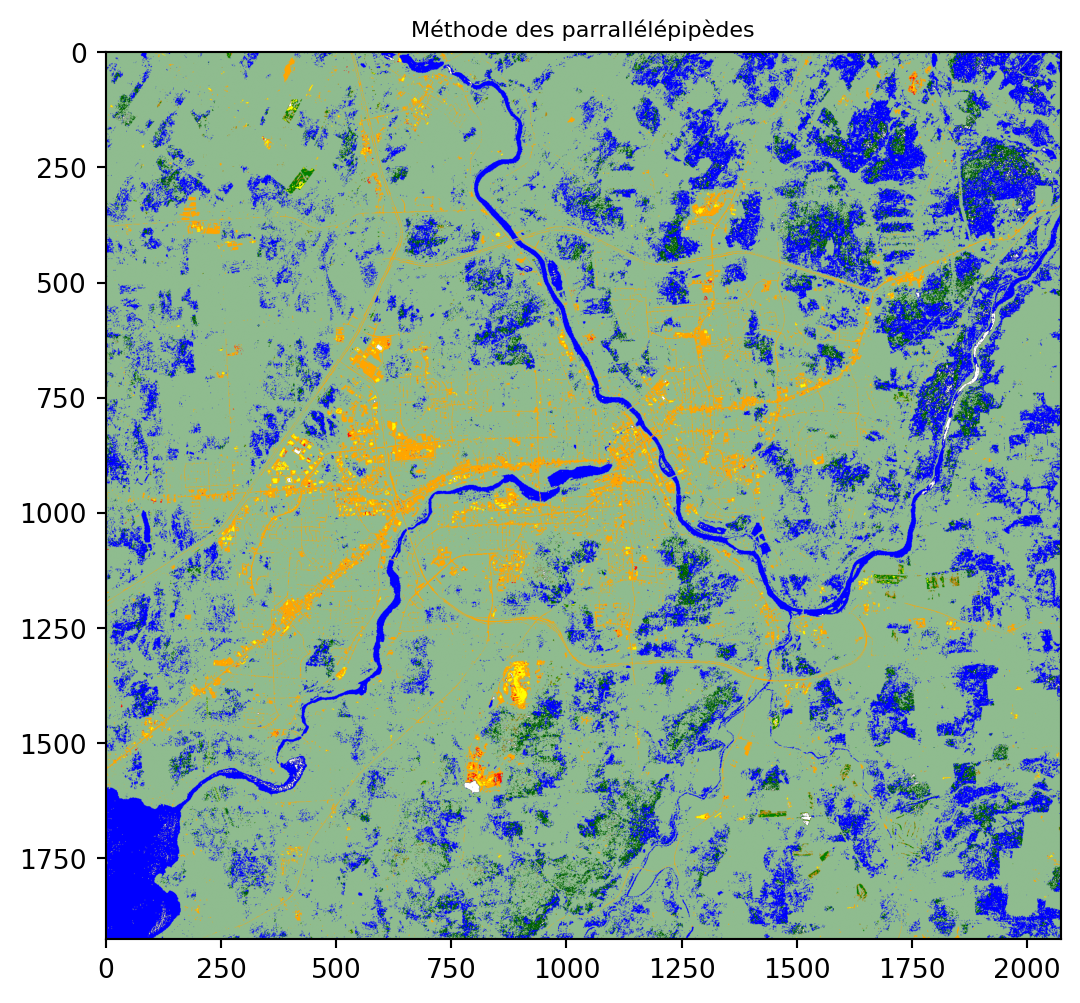
\includegraphics[width=5.625in,height=5.22917in]{05-ClassificationsSupervisees_files/figure-html/cell-22-output-1.png}
\caption{}
\end{figure}

On peut calculer quelques mesures de performance sur l'ensemble
d'entrainement:

\phantomsection\label{2953ed7a}
\phantomsection\label{cb23}
\begin{Shaded}
\begin{Highlighting}[]
\NormalTok{y\_pred}\OperatorTok{=}\NormalTok{ parrallepiped\_predict(clf, X)}
\NormalTok{nom\_classes2}\OperatorTok{=}\NormalTok{ [nom\_classes[c] }\ControlFlowTok{for}\NormalTok{ c }\KeywordTok{in}\NormalTok{ np.unique(y).tolist()]}
\BuiltInTok{print}\NormalTok{(classification\_report(y\_new, y\_pred, target\_names}\OperatorTok{=}\NormalTok{nom\_classes2, zero\_division}\OperatorTok{=}\NormalTok{np.nan))}
\end{Highlighting}
\end{Shaded}

\begin{verbatim}
                       precision    recall  f1-score   support

           Commercial       1.00      0.06      0.11       100
                Foret       1.00      0.09      0.17       100
    Faible_végétation       1.00      0.02      0.04       100
               Sol_nu        nan      0.00      0.00       100
                Roche       0.00      0.00      0.00       100
                Route       0.00      0.00      0.00       100
               Urbain       0.08      0.08      0.08       100
                  Eau       0.83      0.88      0.85       100
    Végétation éparse       1.00      0.01      0.02       100
Roche avec végétation       0.13      1.00      0.23       100

             accuracy                           0.21      1000
            macro avg       0.56      0.21      0.15      1000
         weighted avg       0.56      0.21      0.15      1000
\end{verbatim}

\paragraph{\texorpdfstring{{6.5.1.1} La malédiction de la haute
dimension}{6.5.1.1 La malédiction de la haute dimension}}\label{la-maluxe9diction-de-la-haute-dimension}

Augmenter le nombre de dimension ou de caractéristiques des données
permet de résoudre des problèmes complexes comme la classification
d'image. Cependant, cela amène beaucoup de contraintes sur le volume des
données. Supposons que nous avons N points occupant un segment linéaire
de taille d.~La densité de points est
{\textbackslash(N/d\textbackslash)}. Si nous augmentons le nombre de
dimension D, la densité de points va diminuer exponentiellement en
{\textbackslash(1/d\^{}D\textbackslash)}. Par conséquent, pour garder
une densité constante et donc une bonne estimation des parallélépipèdes,
il nous faudrait augmenter le nombre de points en puissance de D. Ceci
porte le nom de la malédiction de la dimensionnalité
(\emph{dimensionality curse}). En résumé, l'espace vide augmente plus
rapidement que le nombre de données d'entraînement et l'espace des
données devient de plus en plus parcimonieux (\emph{sparse}). Pour
contrecarrer ce problème, on peut sélectionner les meilleures
caractéristiques ou appliquer une réduction de dimension.

\subsubsection{\texorpdfstring{{6.5.2} Plus proches
voisins}{6.5.2 Plus proches voisins}}\label{plus-proches-voisins}

La méthode des plus proches voisins (\emph{K-Nearest-Neighbors} en
Anglais) est certainement la plus simple des méthodes pour classifier
des données. Elle consiste à comparer une nouvelle données avec ces
voisins les plus proches en fonction d'une simple distance Euclidienne.
Si une majorité de ces {\textbackslash(K\textbackslash)} voisins
appartiennent à une classe majoritaire alors cette classe est
sélectionnée. Afin de permettre un vote majoritaire, on choisira un
nombre impair pour la valeur de {\textbackslash(K\textbackslash)}.
Mallgré sa simplicité, cette technique peut devenir assez demandante en
terme de calcul pour un nombre important de points avec un nombre élevé
de dimensions.

Reprensons l'ensemble d'entraînement formé à partir de notre image
RGBNIR précédente:

\phantomsection\label{7dfb466e}
\phantomsection\label{cb25}
\begin{Shaded}
\begin{Highlighting}[]
\NormalTok{df}\OperatorTok{=}\NormalTok{ pd.read\_csv(}\StringTok{\textquotesingle{}sampling\_points.csv\textquotesingle{}}\NormalTok{)}
\CommentTok{\# Extraire la colonne \textquotesingle{}value\textquotesingle{}.}
\CommentTok{\# \textquotesingle{}value\textquotesingle{} est une chaîne de caractères comme représentation d\textquotesingle{}une liste de valeurs.}
\CommentTok{\# Nous devons la convertir en données numériques réelles.}
\NormalTok{X }\OperatorTok{=}\NormalTok{ df[}\StringTok{\textquotesingle{}value\textquotesingle{}}\NormalTok{].}\BuiltInTok{apply}\NormalTok{(}\KeywordTok{lambda}\NormalTok{ x: np.fromstring(x[}\DecValTok{1}\NormalTok{:}\OperatorTok{{-}}\DecValTok{1}\NormalTok{], dtype}\OperatorTok{=}\BuiltInTok{float}\NormalTok{, sep}\OperatorTok{=}\StringTok{\textquotesingle{} \textquotesingle{}}\NormalTok{)).to\_list()}

\CommentTok{\# on obtient une liste de numpy array  qu\textquotesingle{}il faut convertir en un numpy array 2D}
\NormalTok{X}\OperatorTok{=}\NormalTok{ np.array([row.tolist() }\ControlFlowTok{for}\NormalTok{ row }\KeywordTok{in}\NormalTok{ X])}
\NormalTok{idx}\OperatorTok{=}\NormalTok{ X.}\BuiltInTok{sum}\NormalTok{(axis}\OperatorTok{={-}}\DecValTok{1}\NormalTok{)}\OperatorTok{\textgreater{}}\DecValTok{0} \CommentTok{\# il se peut qu\textquotesingle{}il y ait des valeurs erronées}
\NormalTok{X}\OperatorTok{=}\NormalTok{ X[idx,...]}
\NormalTok{y }\OperatorTok{=}\NormalTok{ df[}\StringTok{\textquotesingle{}class\textquotesingle{}}\NormalTok{].to\_numpy()}
\NormalTok{y}\OperatorTok{=}\NormalTok{ y[idx]}
\NormalTok{class\_labels }\OperatorTok{=}\NormalTok{ np.unique(y).tolist() }\CommentTok{\# on cherche à savoir combien de classes uniques}
\NormalTok{n\_classes }\OperatorTok{=} \BuiltInTok{len}\NormalTok{(class\_labels)}
\ControlFlowTok{if} \BuiltInTok{max}\NormalTok{(class\_labels) }\OperatorTok{\textgreater{}}\NormalTok{ n\_classes: }\CommentTok{\# il se peut que certaines classes soit absentes}
\NormalTok{  y\_new}\OperatorTok{=}\NormalTok{ []}
  \ControlFlowTok{for}\NormalTok{ i,l }\KeywordTok{in} \BuiltInTok{enumerate}\NormalTok{(class\_labels):}
\NormalTok{    y\_new.extend([i]}\OperatorTok{*}\BuiltInTok{sum}\NormalTok{(y}\OperatorTok{==}\NormalTok{l))}
\NormalTok{  y\_new }\OperatorTok{=}\NormalTok{ np.array(y\_new)}
\NormalTok{nom\_classes2}\OperatorTok{=}\NormalTok{ [nom\_classes[c] }\ControlFlowTok{for}\NormalTok{ c }\KeywordTok{in}\NormalTok{ np.unique(y).tolist()]}
\end{Highlighting}
\end{Shaded}

Il est important de faire précéder la méthode K-NN par une normalisation
des données de façon à ce que chaque caractéristique soit de moyenne 0
et d'écart-type égale à 1 (on dit parfois que l'on blanchit les
données). Cette normalisation permet à ce que chaque dimension ait le
même poids dans le calcul des distances entre points. Cette opération
porte le nom de \texttt{StandardScaler} dans \texttt{scikit-learn}. On
peut alors former un pipeline de traitement combinant les deux
opérations:

\phantomsection\label{cd7c7777}
\phantomsection\label{cb26}
\begin{Shaded}
\begin{Highlighting}[]
\NormalTok{clf }\OperatorTok{=}\NormalTok{ Pipeline(}
\NormalTok{    steps}\OperatorTok{=}\NormalTok{[(}\StringTok{"scaler"}\NormalTok{, StandardScaler()), (}\StringTok{"knn"}\NormalTok{, KNeighborsClassifier(n\_neighbors}\OperatorTok{=}\DecValTok{1}\NormalTok{))]}
\NormalTok{)}
\end{Highlighting}
\end{Shaded}

Avant d'effectuer un entraînement, on met généralement une portion des
données pour valider les performances:

\phantomsection\label{44d7d104}
\phantomsection\label{cb27}
\begin{Shaded}
\begin{Highlighting}[]
\NormalTok{X\_train, X\_test, y\_train, y\_test }\OperatorTok{=}\NormalTok{ train\_test\_split(X, y\_new, test\_size}\OperatorTok{=}\FloatTok{0.2}\NormalTok{, random\_state}\OperatorTok{=}\DecValTok{0}\NormalTok{)}
\end{Highlighting}
\end{Shaded}

On peut visualiser les frontières de décision du K-NN pour différentes
valeurs de {\textbackslash(K\textbackslash)} lorsque seulement deux
bandes sont utilisées (Rouge et proche infra-rouge ici):

\phantomsection\label{08a687eb}
\begin{verbatim}
Number of mislabeled points out of a total 200 points : 143
Number of mislabeled points out of a total 200 points : 141
Number of mislabeled points out of a total 200 points : 136
Number of mislabeled points out of a total 200 points : 130
\end{verbatim}

\begin{figure}
\centering
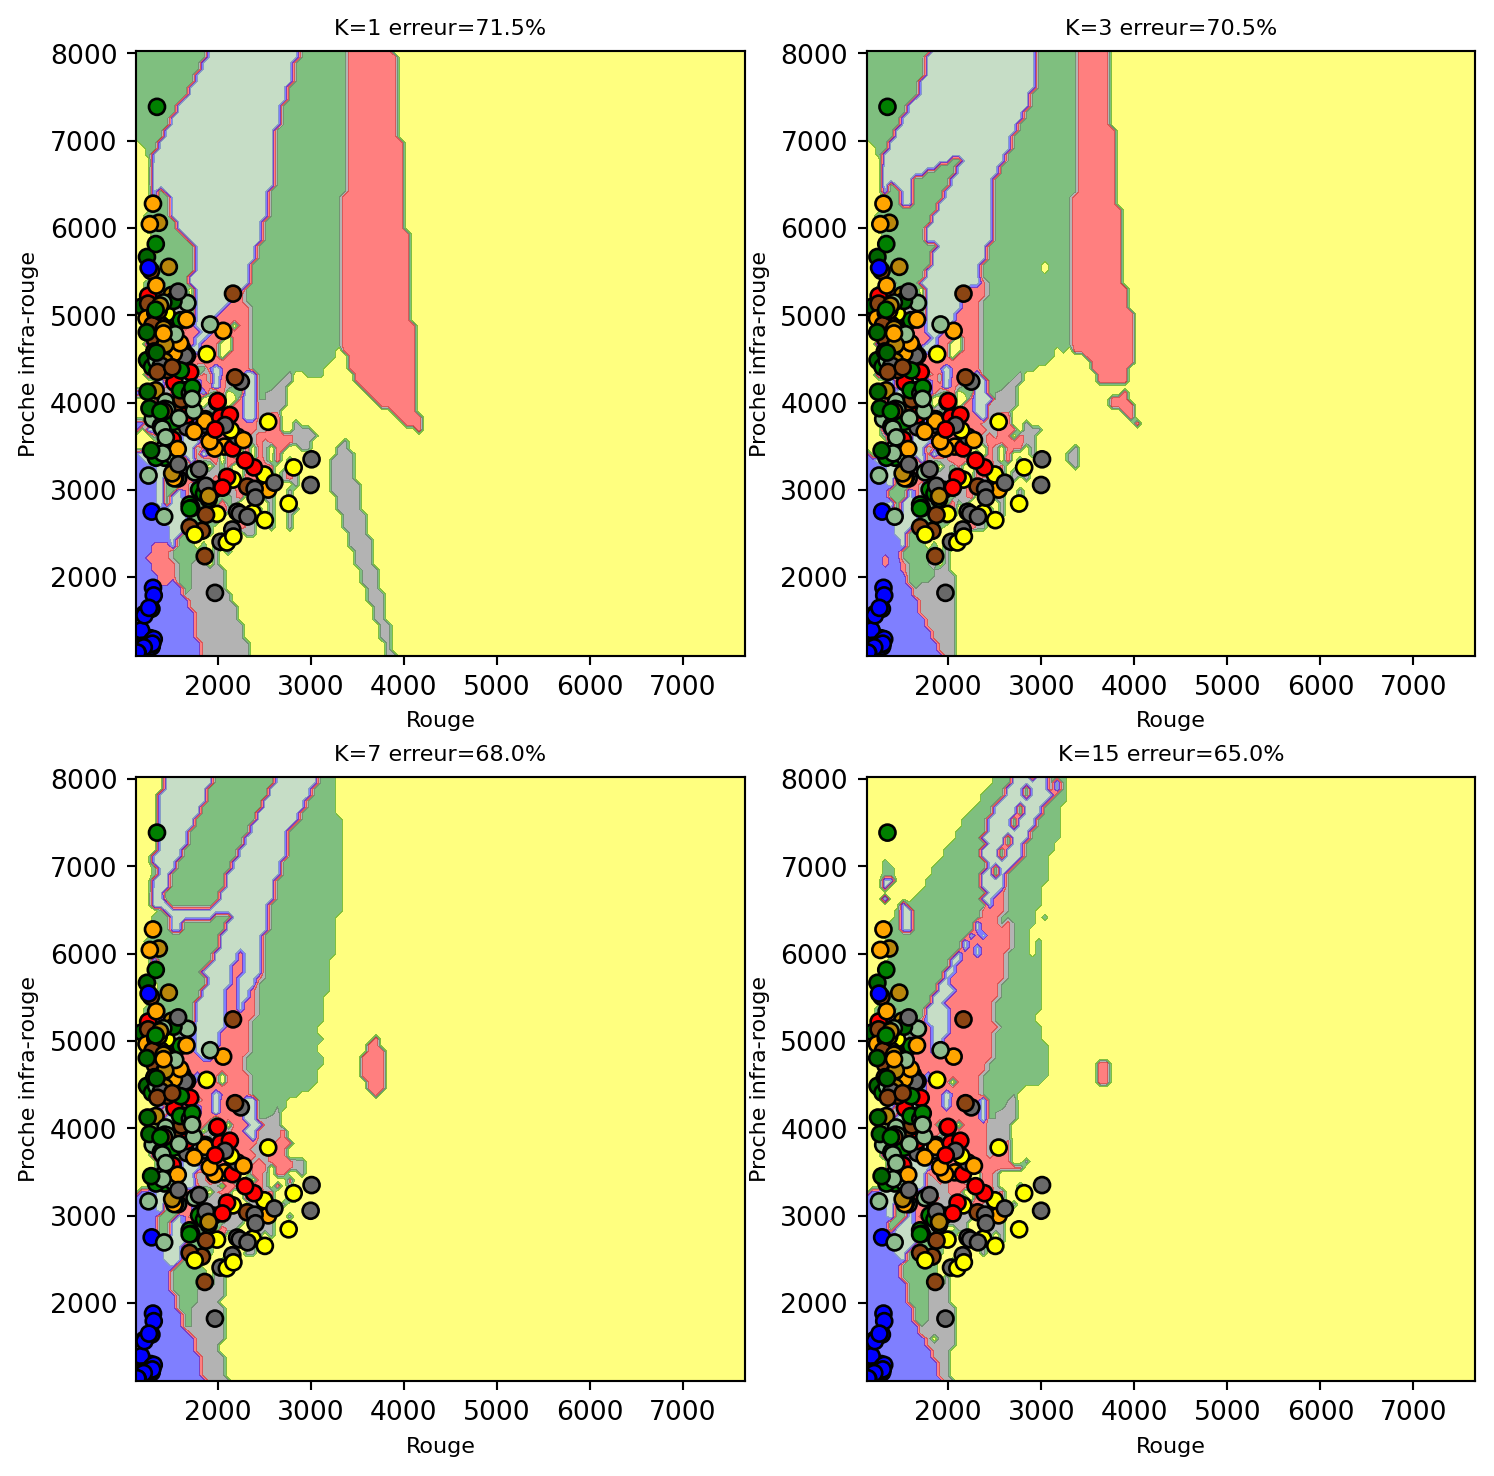
\includegraphics[width=7.78125in,height=7.6875in]{05-ClassificationsSupervisees_files/figure-html/cell-27-output-2.png}
\caption{}
\end{figure}

On peut voir comment les différentes frontières de décision se forment
dans l'espace des bandes Rouge-NIR. L'augmentation de K rend ces
frontières plus complexes et le calcul plus long.

\phantomsection\label{e3b879e0}
\phantomsection\label{cb29}
\begin{Shaded}
\begin{Highlighting}[]
\NormalTok{clf.set\_params(knn\_\_weights}\OperatorTok{=}\StringTok{\textquotesingle{}distance\textquotesingle{}}\NormalTok{, knn\_\_n\_neighbors }\OperatorTok{=} \DecValTok{7}\NormalTok{).fit(X\_train, y\_train)}
\NormalTok{y\_pred }\OperatorTok{=}\NormalTok{ clf.predict(X\_test)}
\BuiltInTok{print}\NormalTok{(}\StringTok{"Nombre de points misclassifiés sur }\SpecialCharTok{\%d}\StringTok{ points : }\SpecialCharTok{\%d}\StringTok{"}
  \OperatorTok{\%}\NormalTok{ (X\_test.shape[}\DecValTok{0}\NormalTok{], (y\_test }\OperatorTok{!=}\NormalTok{ y\_pred).}\BuiltInTok{sum}\NormalTok{()))}
\end{Highlighting}
\end{Shaded}

\begin{verbatim}
Nombre de points misclassifiés sur 200 points : 117
\end{verbatim}

Le rapport de performance est le suivant:

\phantomsection\label{8dce079d}
\phantomsection\label{cb31}
\begin{Shaded}
\begin{Highlighting}[]
\NormalTok{nom\_classes2}\OperatorTok{=}\NormalTok{ [nom\_classes[c] }\ControlFlowTok{for}\NormalTok{ c }\KeywordTok{in}\NormalTok{ np.unique(y).tolist()]}
\BuiltInTok{print}\NormalTok{(classification\_report(y\_test, y\_pred, target\_names}\OperatorTok{=}\NormalTok{nom\_classes2, zero\_division}\OperatorTok{=}\NormalTok{np.nan))}
\end{Highlighting}
\end{Shaded}

\begin{verbatim}
                       precision    recall  f1-score   support

           Commercial       0.38      0.40      0.39        15
                Foret       0.45      0.82      0.58        11
    Faible_végétation       0.29      0.15      0.20        27
               Sol_nu       0.53      0.45      0.49        22
                Roche       0.38      0.26      0.31        23
                Route       0.16      0.17      0.16        18
               Urbain       0.25      0.20      0.22        20
                  Eau       0.96      0.96      0.96        24
    Végétation éparse       0.26      0.53      0.35        15
Roche avec végétation       0.40      0.40      0.40        25

             accuracy                           0.41       200
            macro avg       0.40      0.43      0.40       200
         weighted avg       0.42      0.41      0.40       200
\end{verbatim}

La matrice de confusion peut-être affichée de manière graphique:

\phantomsection\label{fc9200e5}
\phantomsection\label{cb33}
\begin{Shaded}
\begin{Highlighting}[]
\NormalTok{disp}\OperatorTok{=}\NormalTok{ ConfusionMatrixDisplay.from\_predictions(y\_test, y\_pred, display\_labels}\OperatorTok{=}\NormalTok{nom\_classes2, xticks\_rotation}\OperatorTok{=}\StringTok{\textquotesingle{}vertical\textquotesingle{}}\NormalTok{)}
\end{Highlighting}
\end{Shaded}

\begin{figure}
\centering
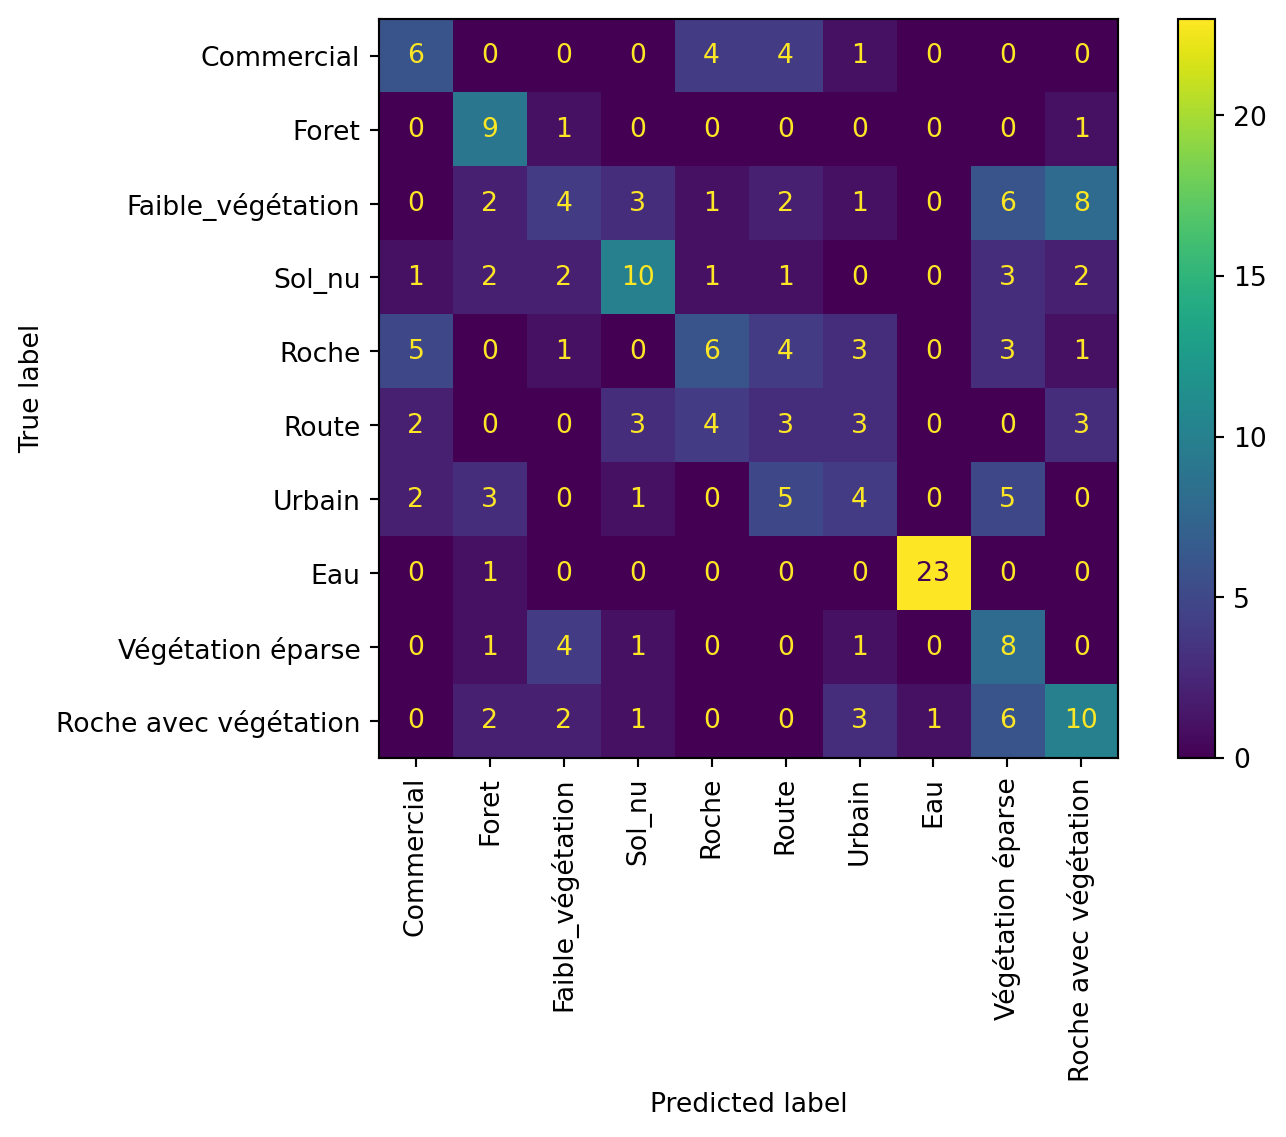
\includegraphics[width=6.69792in,height=5.92708in]{05-ClassificationsSupervisees_files/figure-html/cell-30-output-1.png}
\caption{}
\end{figure}

L'application du modèle (la prédiction) peut se faire sur toute l'image
en transposant l'image sous forme d'une matrice avec Largeur x Hauteur
lignes et 4 colonnes:

\phantomsection\label{afcad211}
\phantomsection\label{cb34}
\begin{Shaded}
\begin{Highlighting}[]
\NormalTok{data\_image}\OperatorTok{=}\NormalTok{ img\_rgbnir.to\_numpy().transpose(}\DecValTok{1}\NormalTok{,}\DecValTok{2}\NormalTok{,}\DecValTok{0}\NormalTok{).reshape(img\_rgbnir.shape[}\DecValTok{1}\NormalTok{]}\OperatorTok{*}\NormalTok{img\_rgbnir.shape[}\DecValTok{2}\NormalTok{],}\DecValTok{4}\NormalTok{)}
\NormalTok{y\_classe}\OperatorTok{=}\NormalTok{ clf.predict(data\_image)}
\NormalTok{y\_classe}\OperatorTok{=}\NormalTok{ y\_classe.reshape(img\_rgbnir.shape[}\DecValTok{1}\NormalTok{],img\_rgbnir.shape[}\DecValTok{2}\NormalTok{])}
\end{Highlighting}
\end{Shaded}

\phantomsection\label{7ca944cb}
\phantomsection\label{cb35}
\begin{Shaded}
\begin{Highlighting}[]
\NormalTok{fig, ax }\OperatorTok{=}\NormalTok{ plt.subplots(nrows}\OperatorTok{=}\DecValTok{1}\NormalTok{, ncols}\OperatorTok{=}\DecValTok{1}\NormalTok{, figsize}\OperatorTok{=}\NormalTok{(}\DecValTok{8}\NormalTok{, }\DecValTok{6}\NormalTok{))}
\NormalTok{plt.imshow(y\_classe, cmap}\OperatorTok{=}\NormalTok{cmap\_classes2)}
\NormalTok{ax.set\_title(}\StringTok{"Carte d\textquotesingle{}occupation des sols avec K{-}NN"}\NormalTok{, fontsize}\OperatorTok{=}\StringTok{"small"}\NormalTok{)}
\NormalTok{plt.show()}
\end{Highlighting}
\end{Shaded}

\begin{figure}
\centering
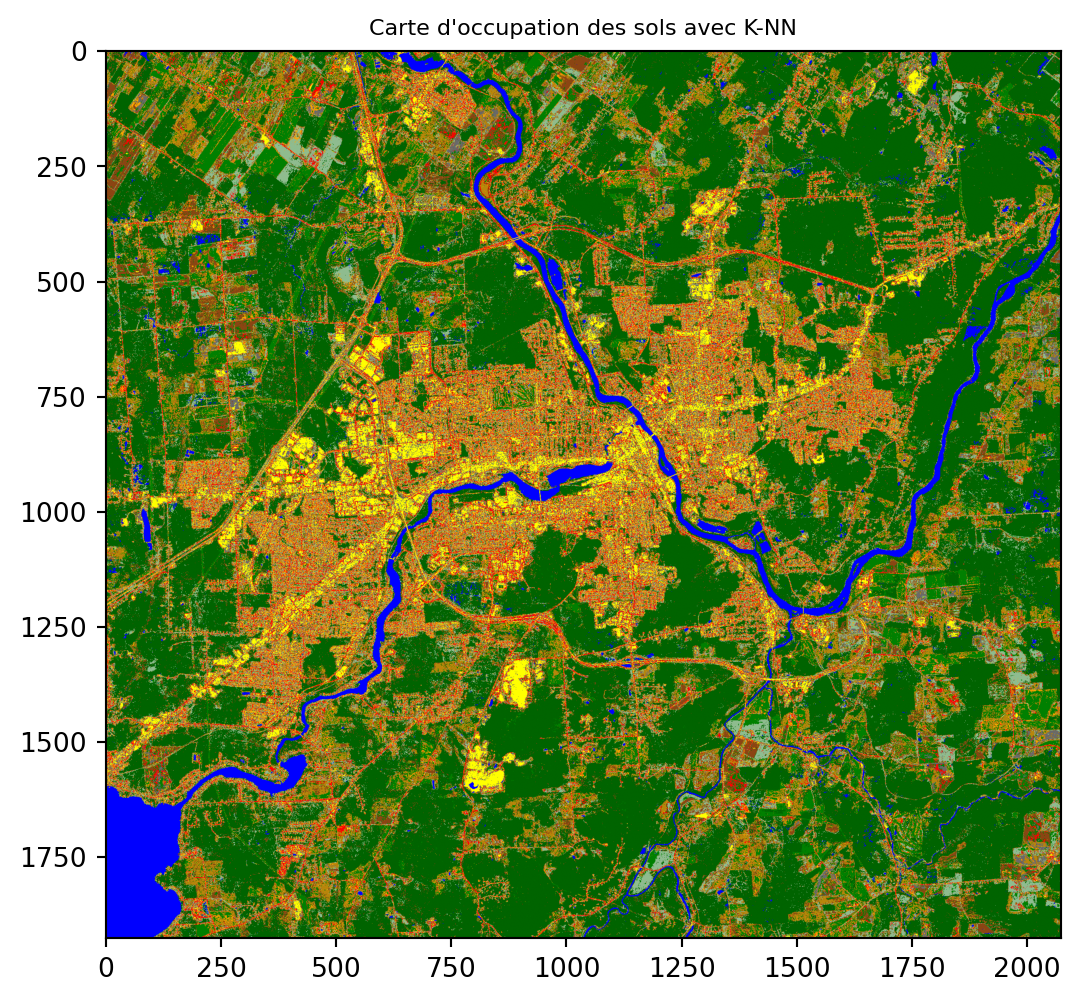
\includegraphics[width=5.625in,height=5.21875in]{05-ClassificationsSupervisees_files/figure-html/cell-32-output-1.png}
\caption{}
\end{figure}

\subsubsection{\texorpdfstring{{6.5.3} Méthodes par arbre de
décision}{6.5.3 Méthodes par arbre de décision}}\label{muxe9thodes-par-arbre-de-duxe9cision}

La méthode par arbre de décision consiste à contruire une cascade de
règles de décision sur chaque caractéristique du jeu de donnée. On
pourra trouver plus de détails dans la documentation de
\texttt{scikit-learn}
(\href{https://scikit-learn.org/stable/modules/tree.html}{Decision
Trees}). Les arbres de décision on tendance à sur-apprendre surtout si
le nombre de dimensions est élevé. Il est donc conseillé d'avoir un bon
ratio entre le nombre d'échantillons et le nombre de dimensions.

\phantomsection\label{694d96e4}
\phantomsection\label{cb36}
\begin{Shaded}
\begin{Highlighting}[]
\NormalTok{X\_train, X\_test, y\_train, y\_test }\OperatorTok{=}\NormalTok{ train\_test\_split(X, y, test\_size}\OperatorTok{=}\FloatTok{0.2}\NormalTok{, random\_state}\OperatorTok{=}\DecValTok{0}\NormalTok{)}
\end{Highlighting}
\end{Shaded}

\phantomsection\label{a47dcffd}
\begin{verbatim}
Number of mislabeled points out of a total 200 points : 167
Number of mislabeled points out of a total 200 points : 154
Number of mislabeled points out of a total 200 points : 143
Number of mislabeled points out of a total 200 points : 128
\end{verbatim}

\begin{figure}
\centering
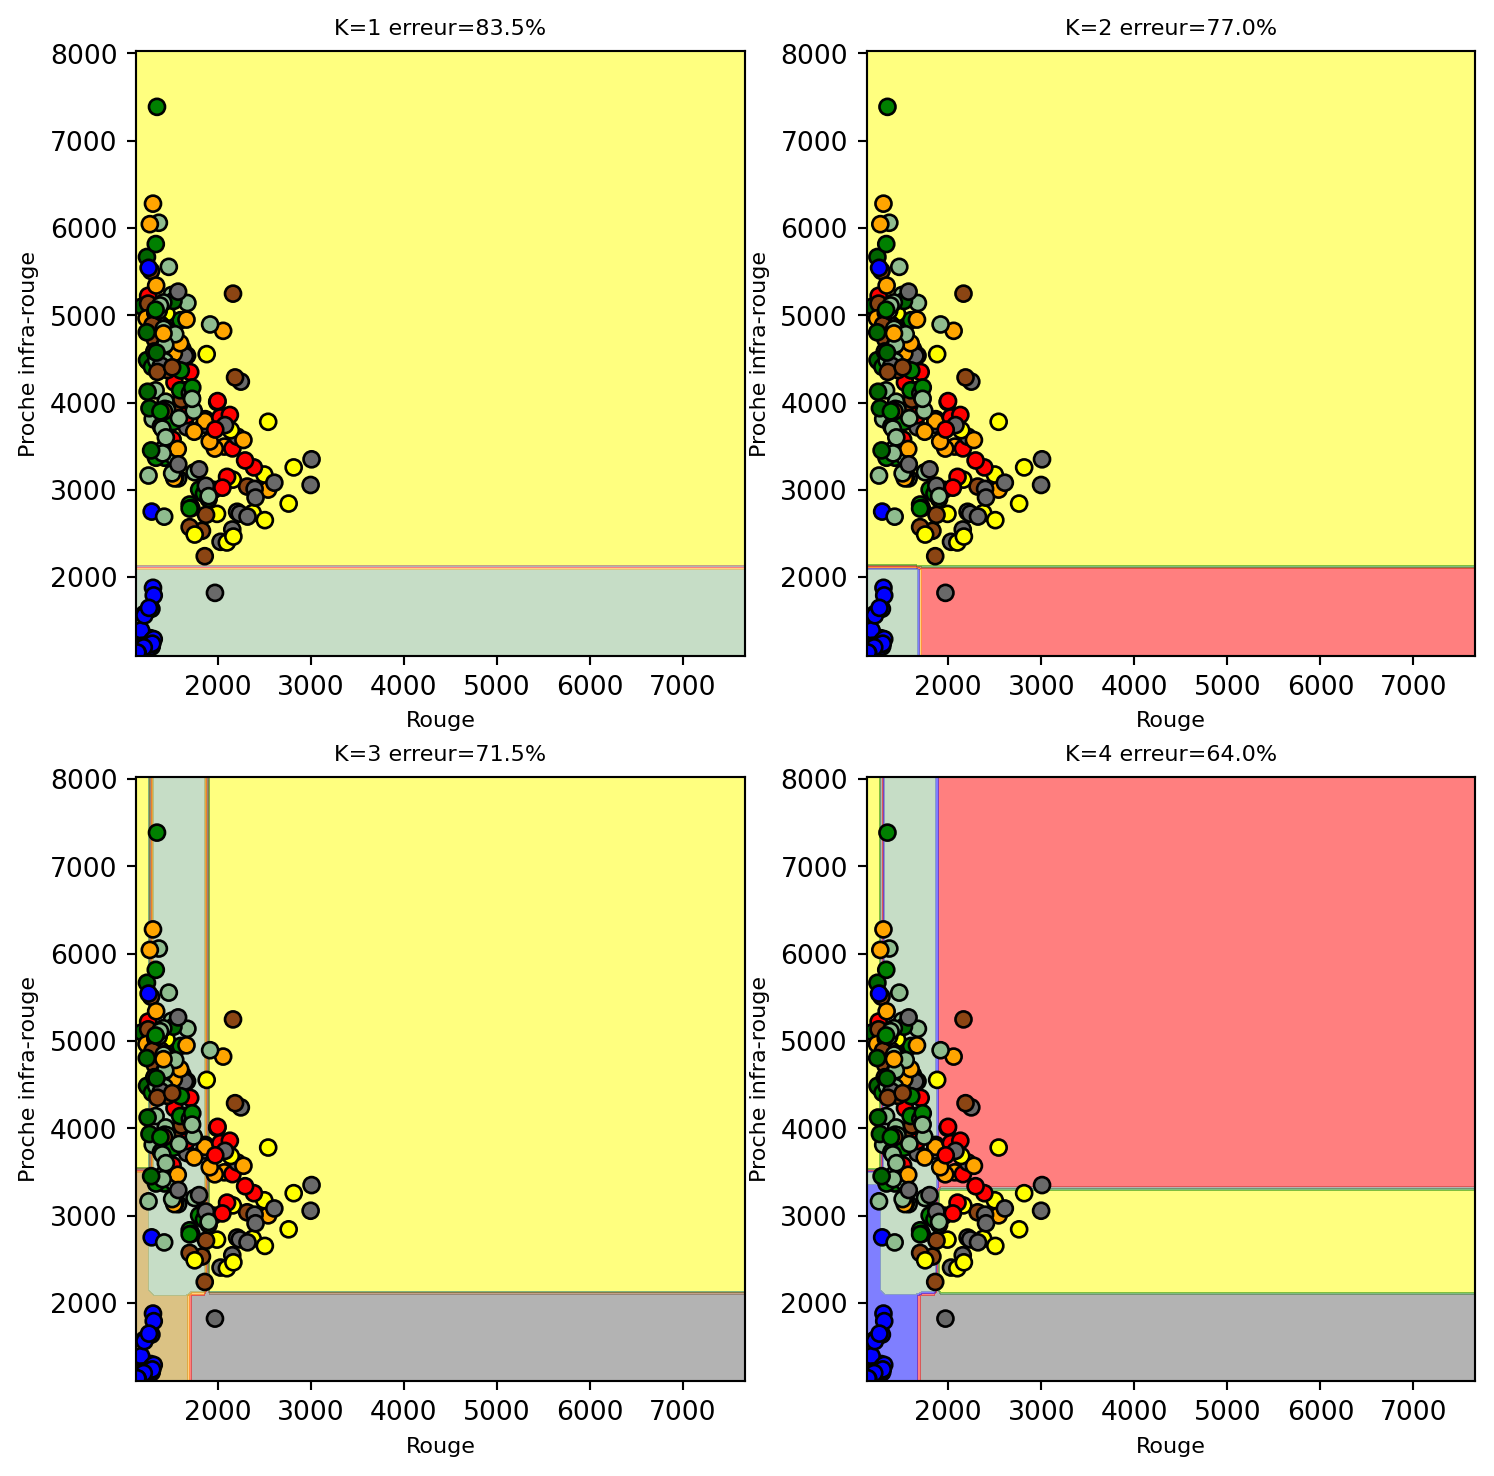
\includegraphics[width=7.78125in,height=7.6875in]{05-ClassificationsSupervisees_files/figure-html/cell-34-output-2.png}
\caption{}
\end{figure}

On peut observer que les frontières de décision sont formées d'un
ensemble de plans simple. Chaque plan étant issu d'une règle de décison
formé d'un seuil sur chacune des dimensions. On entraine un arbre de
décision avec une profondeur maximale de 5:

\phantomsection\label{851bd868}
\phantomsection\label{cb38}
\begin{Shaded}
\begin{Highlighting}[]
\NormalTok{clf }\OperatorTok{=}\NormalTok{ tree.DecisionTreeClassifier(max\_depth}\OperatorTok{=}\DecValTok{5}\NormalTok{)}
\NormalTok{clf.fit(X\_train, y\_train)}
\NormalTok{y\_pred }\OperatorTok{=}\NormalTok{ clf.predict(X\_test)}
\BuiltInTok{print}\NormalTok{(}\StringTok{"Nombre de points misclassifiés sur }\SpecialCharTok{\%d}\StringTok{ points : }\SpecialCharTok{\%d}\StringTok{"}
  \OperatorTok{\%}\NormalTok{ (X\_test.shape[}\DecValTok{0}\NormalTok{], (y\_test }\OperatorTok{!=}\NormalTok{ y\_pred).}\BuiltInTok{sum}\NormalTok{()))}
\end{Highlighting}
\end{Shaded}

\begin{verbatim}
Nombre de points misclassifiés sur 200 points : 130
\end{verbatim}

Le rapport de performance et la matrice de confusion:

\phantomsection\label{62023190}
\begin{verbatim}
                       precision    recall  f1-score   support

           Commercial       0.37      0.47      0.41        15
                Foret       0.57      0.73      0.64        11
    Faible_végétation       0.19      0.19      0.19        27
               Sol_nu       0.57      0.18      0.28        22
                Roche       0.40      0.09      0.14        23
                Route       0.32      0.44      0.37        18
               Urbain        nan      0.00      0.00        20
                  Eau       0.95      0.79      0.86        24
    Végétation éparse        nan      0.00      0.00        15
Roche avec végétation       0.20      0.68      0.31        25

             accuracy                           0.35       200
            macro avg       0.45      0.36      0.32       200
         weighted avg       0.44      0.35      0.31       200
\end{verbatim}

\phantomsection\label{c5af5511}
\begin{figure}
\centering
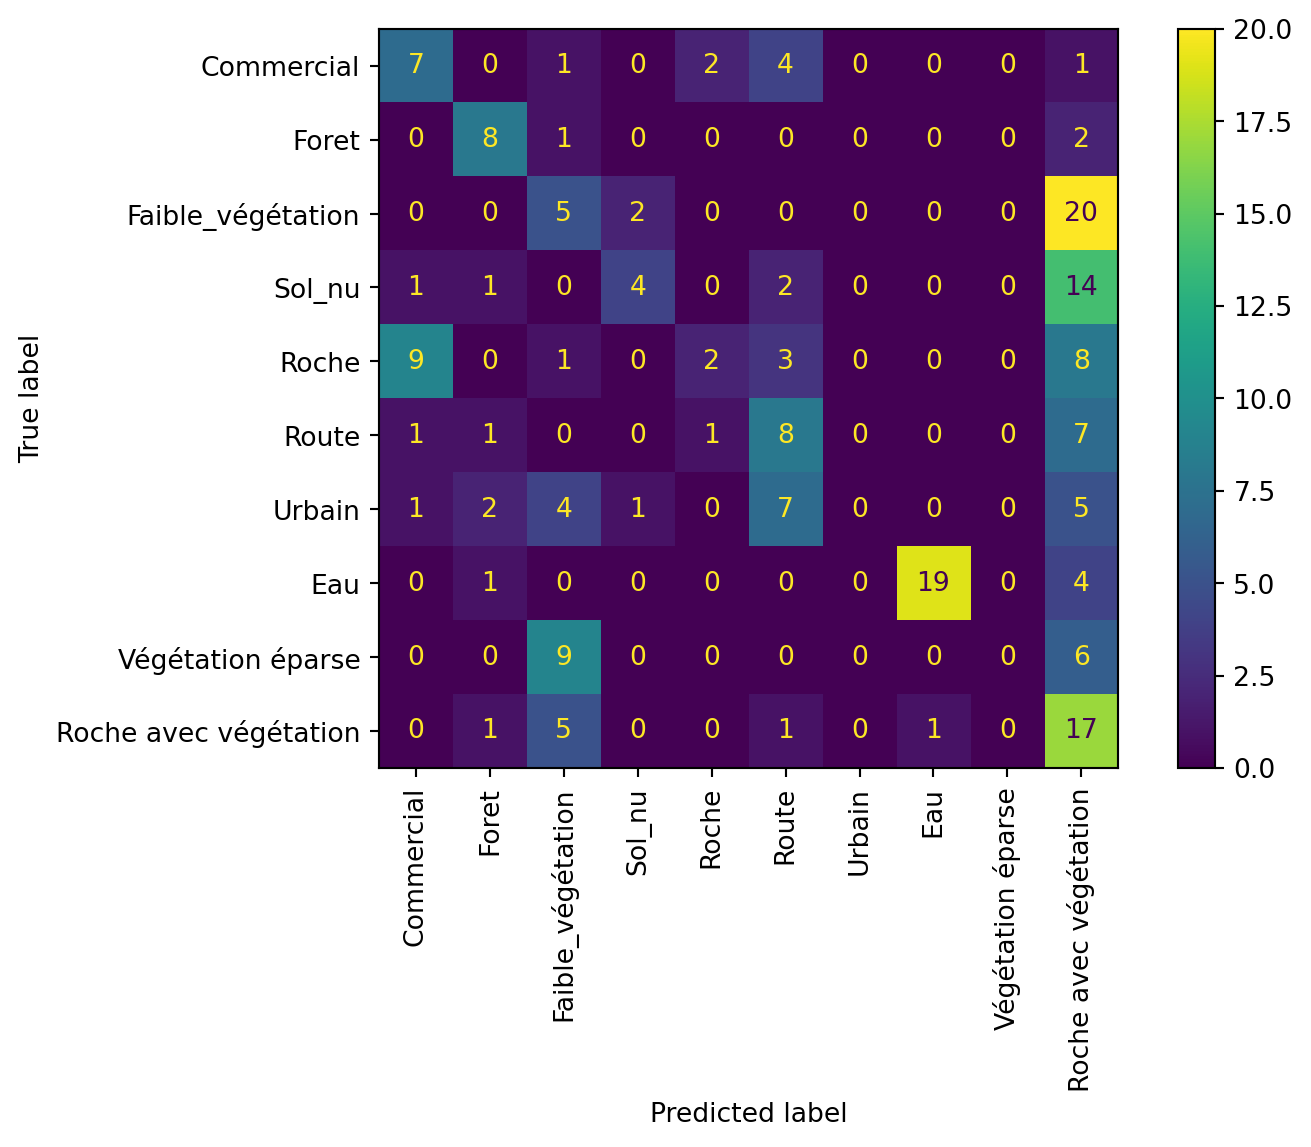
\includegraphics[width=6.83333in,height=5.97917in]{05-ClassificationsSupervisees_files/figure-html/cell-37-output-1.png}
\caption{}
\end{figure}

L'application du modèle (la prédiction) peut se faire sur toute l'image
en transposant l'image sous forme d'une matrice avec Largeur x Hauteur
lignes et 4 colonnes:

\phantomsection\label{248842f3}
\begin{figure}
\centering
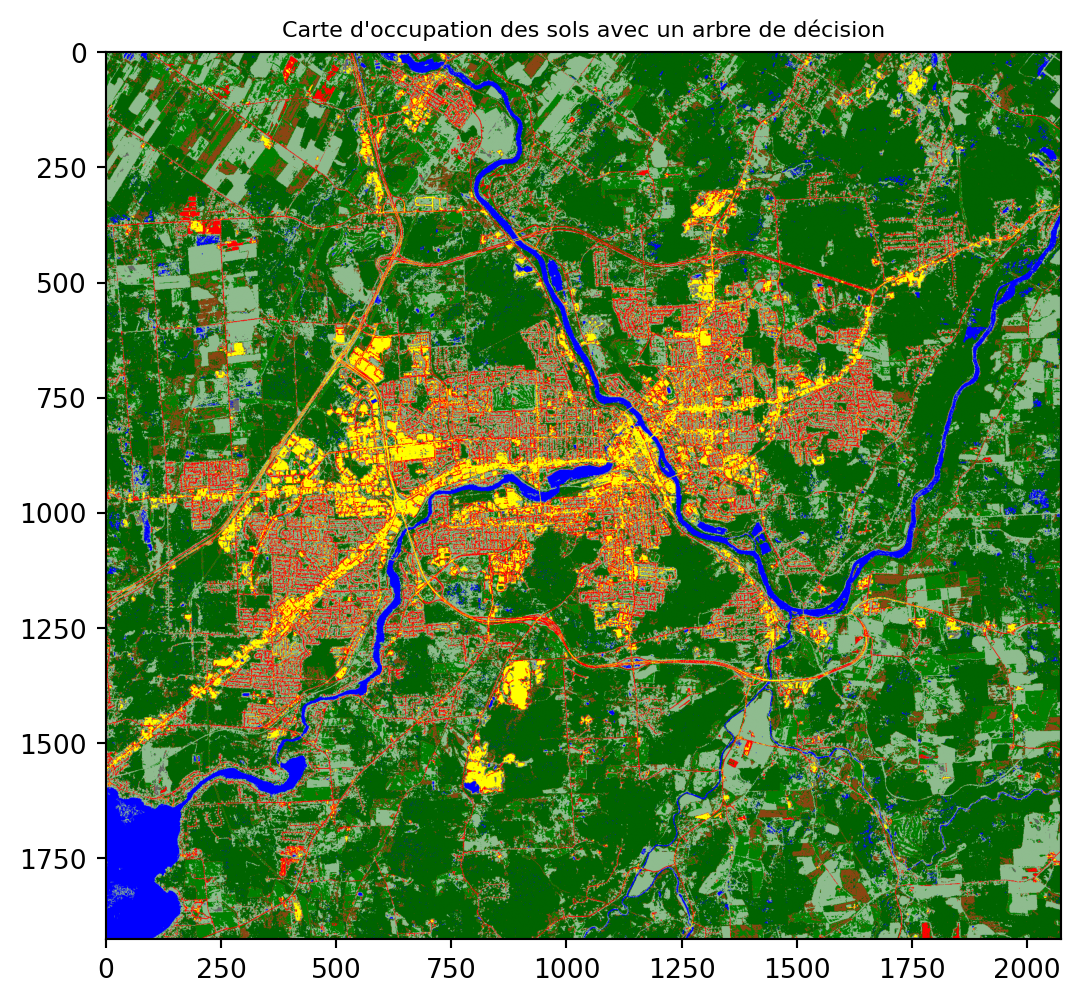
\includegraphics[width=5.625in,height=5.22917in]{05-ClassificationsSupervisees_files/figure-html/cell-39-output-1.png}
\caption{}
\end{figure}

Il est possible de visualiser l'arbre mais cela contient beaucoup
d'information

\phantomsection\label{3163f0dc}
\phantomsection\label{cb41}
\begin{Shaded}
\begin{Highlighting}[]
\NormalTok{fig, ax }\OperatorTok{=}\NormalTok{ plt.subplots(nrows}\OperatorTok{=}\DecValTok{1}\NormalTok{, ncols}\OperatorTok{=}\DecValTok{1}\NormalTok{, figsize}\OperatorTok{=}\NormalTok{(}\DecValTok{8}\NormalTok{, }\DecValTok{6}\NormalTok{))}
\NormalTok{tree.plot\_tree(clf, max\_depth}\OperatorTok{=}\DecValTok{1}\NormalTok{)}
\end{Highlighting}
\end{Shaded}

\begin{verbatim}
[Text(0.5, 0.8333333333333334, 'x[3] <= 2139.0\ngini = 0.9\nsamples = 800\nvalue = [85, 89, 73, 78, 77, 82, 80, 76, 85, 75]'),
 Text(0.25, 0.5, 'x[2] <= 1714.0\ngini = 0.055\nsamples = 71\nvalue = [0, 0, 0, 0, 1, 0, 0, 69, 0, 1]'),
 Text(0.375, 0.6666666666666667, 'True  '),
 Text(0.125, 0.16666666666666666, '\n  (...)  \n'),
 Text(0.375, 0.16666666666666666, '\n  (...)  \n'),
 Text(0.75, 0.5, 'x[2] <= 1277.0\ngini = 0.89\nsamples = 729\nvalue = [85.0, 89.0, 73.0, 78.0, 76.0, 82.0, 80.0, 7.0, 85.0\n74.0]'),
 Text(0.625, 0.6666666666666667, '  False'),
 Text(0.625, 0.16666666666666666, '\n  (...)  \n'),
 Text(0.875, 0.16666666666666666, '\n  (...)  \n')]
\end{verbatim}

\begin{figure}
\centering
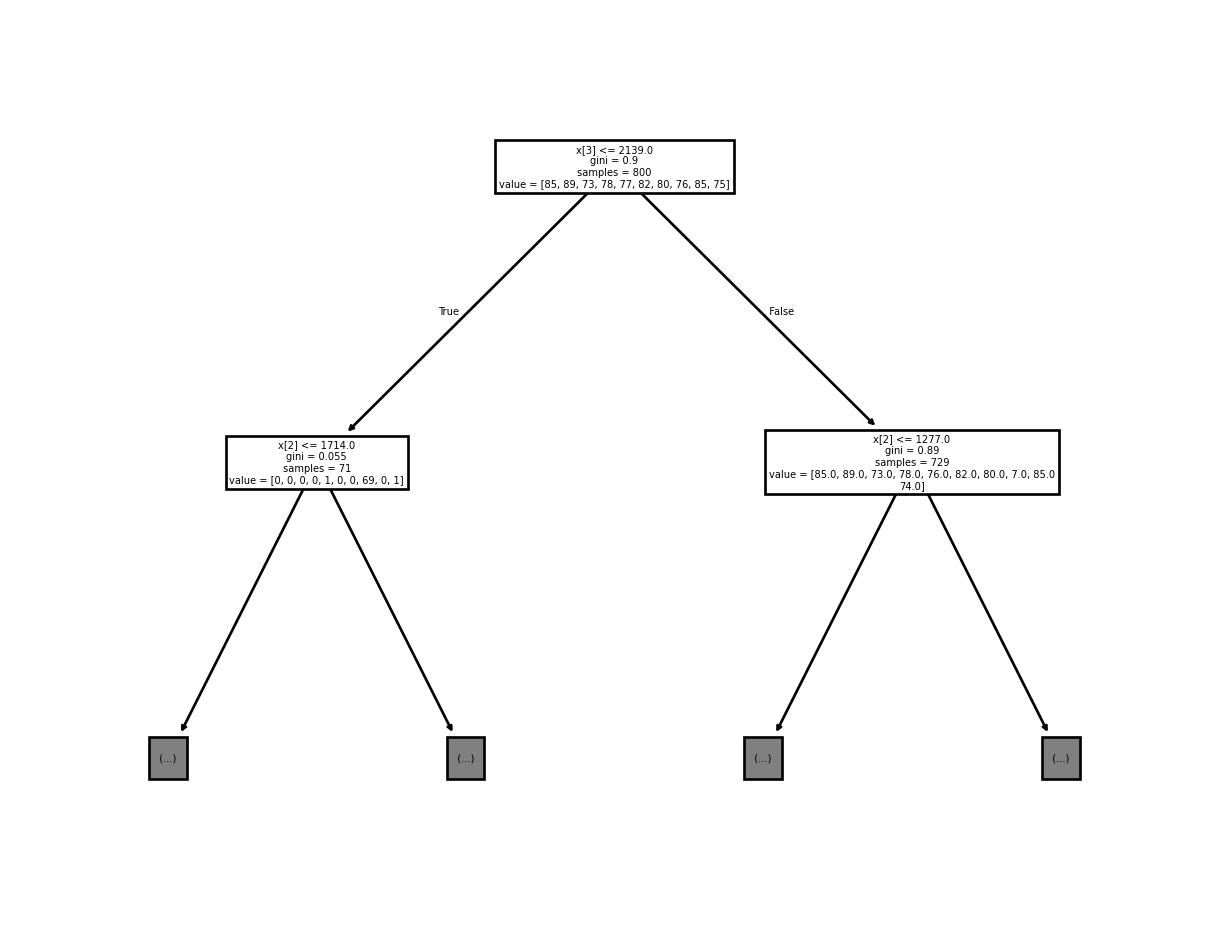
\includegraphics[width=6.39583in,height=4.82292in]{05-ClassificationsSupervisees_files/figure-html/cell-40-output-2.png}
\caption{}
\end{figure}

\subsection{\texorpdfstring{{6.6} Méthodes
paramétriques}{6.6 Méthodes paramétriques}}\label{muxe9thodes-paramuxe9triques}

Les méthodes paramétriques se basent sur des modélisations statistiques
des données pour permettre une classification. Contraitement au méthodes
non paramétriques, elles ont un nombre fixe de paramètres qui ne dépend
pas de la taille du jeu de données. Par contre, des hypothèses sont
faites sur le comportement statistique des données. La classification
consiste alors à trouver la classe la plus vraisemblable dont le modèle
statistique décrit le mieux les valeurs observées. L'ensemble
d'entraînement permettra alors de calculer les paramètres de chaque
Gaussienne pour chacune des classes d'intérêt.

\subsubsection{\texorpdfstring{{6.6.1} Méthode Bayésienne
naïve}{6.6.1 Méthode Bayésienne naïve}}\label{muxe9thode-bayuxe9sienne-nauxefve}

La méthode Bayésienne naïve Gaussienne consiste faire des hypothèses
simplificatrices sur les données, en particulier l'indépendance des
données et des dimensions. Ceci permet un calcul plus simple.

\phantomsection\label{4b596e68}
\phantomsection\label{cb43}
\begin{Shaded}
\begin{Highlighting}[]
\ImportTok{from}\NormalTok{ sklearn.naive\_bayes }\ImportTok{import}\NormalTok{ GaussianNB}
\NormalTok{gnb }\OperatorTok{=}\NormalTok{ GaussianNB()}
\NormalTok{y\_pred }\OperatorTok{=}\NormalTok{ gnb.fit(X\_train, y\_train).predict(X\_test)}
\BuiltInTok{print}\NormalTok{(}\StringTok{"Nombre de points erronés sur }\SpecialCharTok{\%d}\StringTok{ points : }\SpecialCharTok{\%d}\StringTok{"}
      \OperatorTok{\%}\NormalTok{ (X\_test.shape[}\DecValTok{0}\NormalTok{], (y\_test }\OperatorTok{!=}\NormalTok{ y\_pred).}\BuiltInTok{sum}\NormalTok{()))}
\end{Highlighting}
\end{Shaded}

\begin{verbatim}
Nombre de points erronés sur 200 points : 131
\end{verbatim}

\phantomsection\label{ae124bd9}
\begin{figure}
\centering
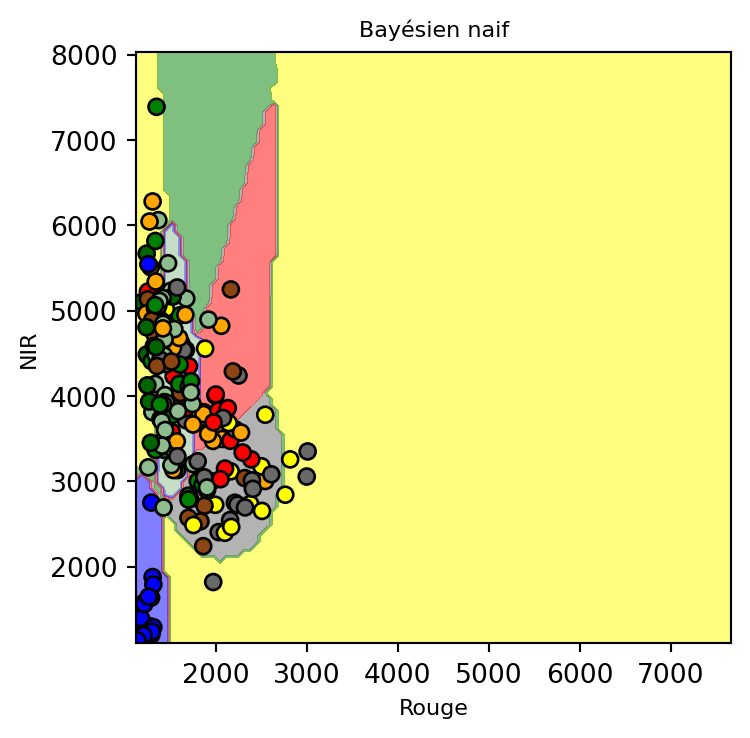
\includegraphics[width=3.90625in,height=3.84375in]{05-ClassificationsSupervisees_files/figure-html/cell-42-output-1.png}
\caption{}
\end{figure}

On peut observer que les frontières de décision sont beaucoup plus
régulières que pour K-NN.

\phantomsection\label{e321431e}
\phantomsection\label{cb45}
\begin{Shaded}
\begin{Highlighting}[]
\NormalTok{gnb.fit(X\_train, y\_train)}
\NormalTok{y\_pred }\OperatorTok{=}\NormalTok{ gnb.predict(X\_test)}
\BuiltInTok{print}\NormalTok{(}\StringTok{"Nombre de points misclassifiés sur }\SpecialCharTok{\%d}\StringTok{ points : }\SpecialCharTok{\%d}\StringTok{"}
  \OperatorTok{\%}\NormalTok{ (X\_test.shape[}\DecValTok{0}\NormalTok{], (y\_test }\OperatorTok{!=}\NormalTok{ y\_pred).}\BuiltInTok{sum}\NormalTok{()))}
\end{Highlighting}
\end{Shaded}

\begin{verbatim}
Nombre de points misclassifiés sur 200 points : 131
\end{verbatim}

De la même manière, la prédiction peut s'appliquer sur toute l'image:

\phantomsection\label{1b9ddbf0}
\begin{figure}
\centering
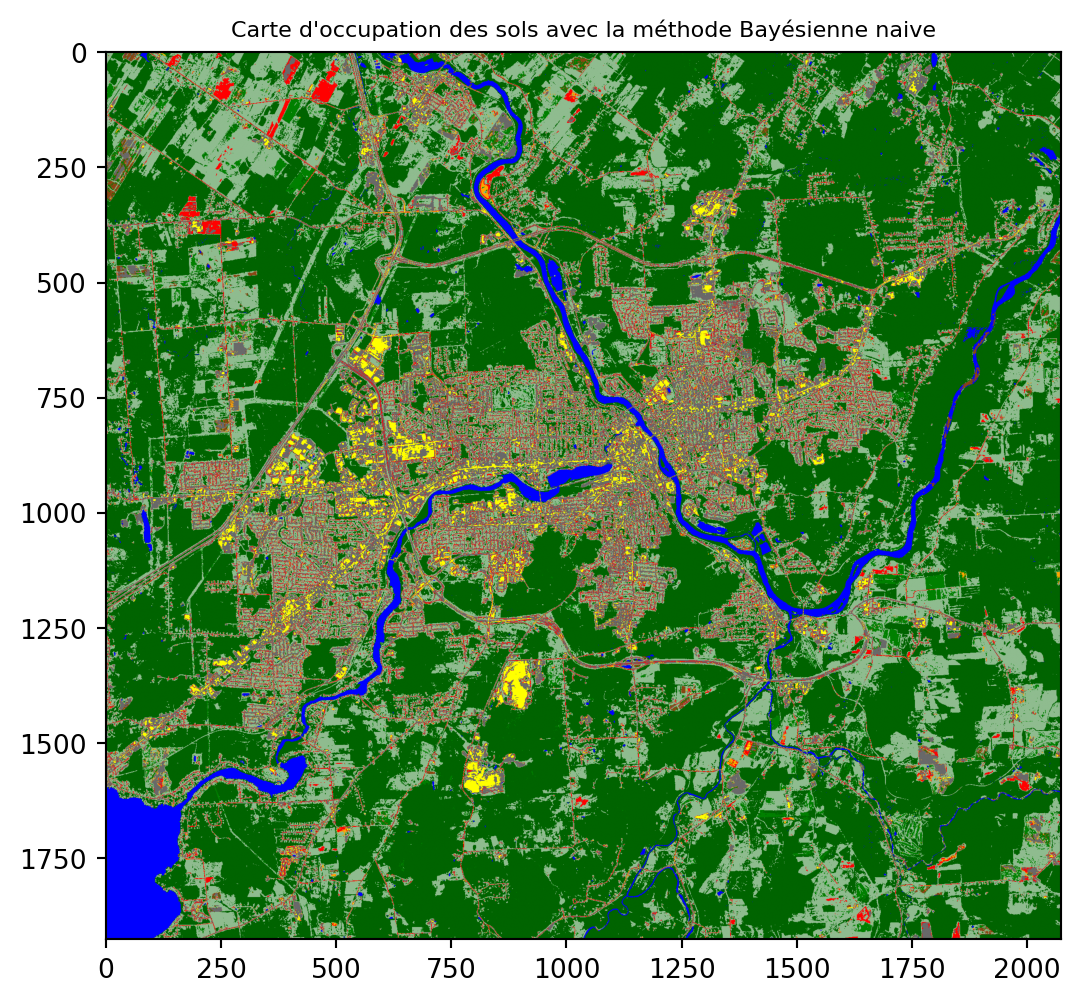
\includegraphics[width=5.625in,height=5.22917in]{05-ClassificationsSupervisees_files/figure-html/cell-44-output-1.png}
\caption{}
\end{figure}

\subsubsection{\texorpdfstring{{6.6.2} Analyse Discriminante Quadratique
(ADQ)}{6.6.2 Analyse Discriminante Quadratique (ADQ)}}\label{analyse-discriminante-quadratique-adq}

L'analyse discriminante quadratique peut-être vue comme une
généralisation de l'approche Bayésienne naive qui suppose des modèles
Gaussiens indépendants pour chaque dimension et chaque point. Ici, on va
considérer un modèle Gaussien multivarié.

\phantomsection\label{e513ddf0}
\phantomsection\label{cb47}
\begin{Shaded}
\begin{Highlighting}[]
\NormalTok{qda }\OperatorTok{=}\NormalTok{ QuadraticDiscriminantAnalysis(store\_covariance}\OperatorTok{=}\VariableTok{True}\NormalTok{)}
\NormalTok{qda.fit(X\_train, y\_train)}
\NormalTok{y\_pred }\OperatorTok{=}\NormalTok{ qda.predict(X\_test)}
\BuiltInTok{print}\NormalTok{(}\StringTok{"Nombre de points misclassifiés sur }\SpecialCharTok{\%d}\StringTok{ points : }\SpecialCharTok{\%d}\StringTok{"}
  \OperatorTok{\%}\NormalTok{ (X\_test.shape[}\DecValTok{0}\NormalTok{], (y\_test }\OperatorTok{!=}\NormalTok{ y\_pred).}\BuiltInTok{sum}\NormalTok{()))}
\end{Highlighting}
\end{Shaded}

\begin{verbatim}
Nombre de points misclassifiés sur 200 points : 124
\end{verbatim}

Les Gaussiennes multivariées peuvent être visualiser sous forme
d'éllipses décrivant le domaine des valeurs de chaque classe:

\phantomsection\label{6dfabd0f}
\begin{figure}
\centering
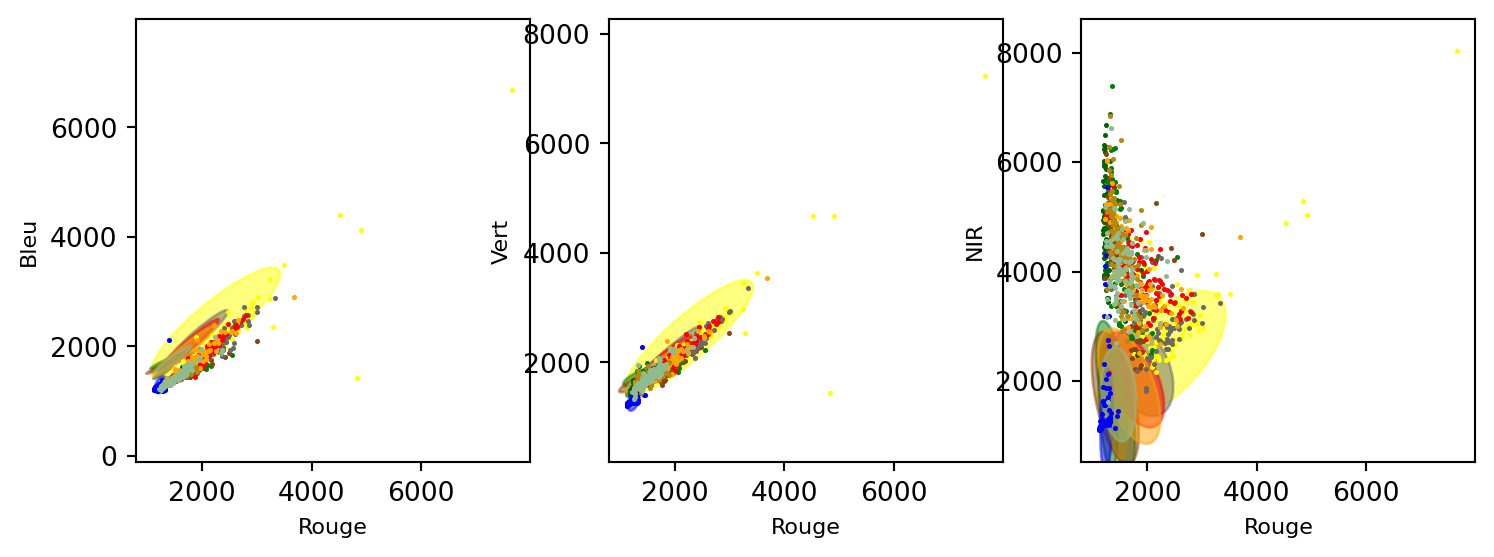
\includegraphics[width=7.78125in,height=2.90625in]{05-ClassificationsSupervisees_files/figure-html/cell-46-output-1.png}
\caption{}
\end{figure}

De la même manière, la prédiction peut s'appliquer sur toute l'image:

\phantomsection\label{b9ece539}
\begin{figure}
\centering
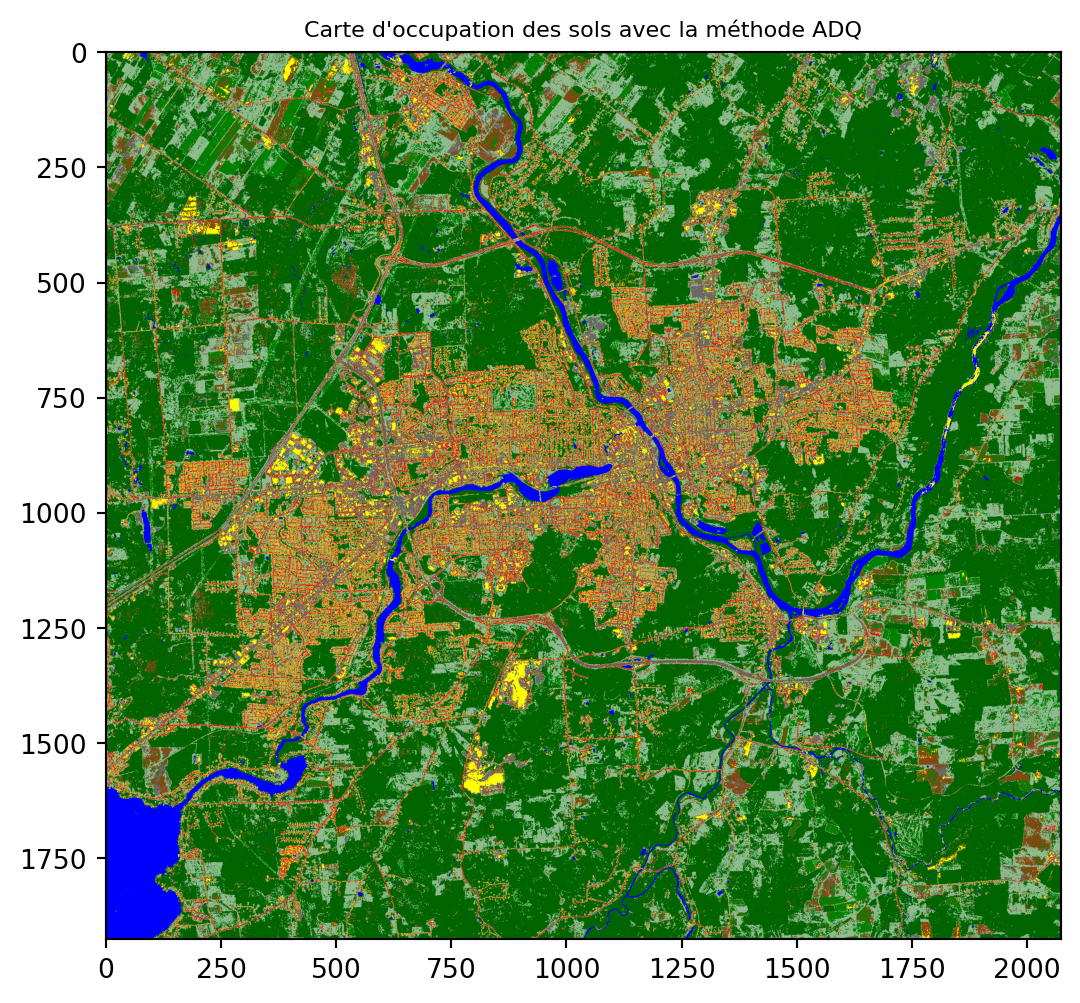
\includegraphics[width=5.625in,height=5.22917in]{05-ClassificationsSupervisees_files/figure-html/cell-47-output-1.png}
\caption{}
\end{figure}

\end{document}
